\documentclass[hyperref={pdfpagelabels=false},compress]{beamer}
\usepackage{lmodern}
\usepackage[utf8]{inputenc}
\usepackage{amssymb}
\usepackage{amsmath}
\usepackage{tikz}
\usepackage{tkz-euclide}
\usepackage[percent]{overpic}
\usepackage{multimedia}
\usepackage{pgfplots}
\usepgfplotslibrary{patchplots}
\graphicspath{{Pictures/}}
\usetikzlibrary{arrows,calc,intersections,shapes,backgrounds,shadows,automata,patterns}
\usetheme{Berlin}
\definecolor{UniRed}{RGB}{255,0,0}
\definecolor{UniWhite}{RGB}{255,255,255}
\definecolor{PresiBlue}{RGB}{50,57,171}
\setbeamercolor{eecks} {bg=UniRed, fg=UniWhite}
\setbeamercolor{presinative}{bg=PresiBlue, fg=UniWhite}

% Layer tikz definitions
\tikzstyle{block} = [
	rectangle, draw, fill=blue!20,
	text width=20em, text centered,
	rounded corners, minimum height=4em,
	node distance=2.5cm]

\tikzstyle{block-active} = [
	rectangle, draw, fill=green!20,
	text width=20em, text centered,
	rounded corners, minimum height=4em,
	node distance=2.5cm]

\tikzstyle{cloud} = [draw, ellipse,fill=red!20, node distance=2cm, minimum height=2em]

\tikzstyle{line} = [draw, ->, >=stealth', ultra thick]
\tikzstyle{dline} = [draw, <->, >=stealth', ultra thick]

% Router tikz definitions
\def\robot at (#1,#2) {
	\draw[fill=red] (#1,#2) circle (0.35);
	\draw[fill=blue] (#1,#2)++(0.15,0) circle (0.1);
}
\def\robotr at (#1,#2) {
	\draw[fill=red] (#1,#2) circle (0.35);
	\draw[fill=blue] (#1,#2)++(0,0.15) circle (0.1);
}
\def\goal at (#1,#2) {
	\draw[red,line width=8pt] (#1,#2)+(-.35,-.35)--+(.35,.35) +(-0.35,0.35)--+(.35,-.35);
}
\def\goalHelp at (#1,#2) {
	\draw[green!80!blue,line width=8pt] (#1,#2)+(-.35,-.35)--+(.35,.35) +(-0.35,0.35)--+(.35,-.35);
}
\def\ball at (#1,#2) {
	\draw [thin, fill=white] (#1,#2) circle (0.15);
	\shade[ball color=blue!10!white,opacity=0.50] (#1,#2) circle (0.15);
}
\tikzstyle{edge} = [draw,line width=24pt,-,gray]
\tikzstyle{selected edge} = [draw,line width=24pt,-,green]
\tikzstyle{ignored edge} = [draw,line width=24pt,-,red!50!white]
\tikzstyle{obstacle} = [draw,very thick,circle,minimum size=20pt,shading=radial,outer color=black!80!white,inner color=white]
\tikzstyle{selected obstacle} = [draw,very thick,circle,fill=blue!20!white,minimum size=20pt]
\tikzset{cross/.style={cross out, draw=green, minimum size=2*(#1-\pgflinewidth), inner sep=0pt, outer sep=0pt}, cross/.default={3pt}}

% Title
\title{\textsc{RoboSoccer} Project Plan}
\author[Hofbauer, Jiang, Meyer, Schmidt, Wirnshofer]{
  Markus~Hofbauer \and
  He~Jiang \and
  Kevin~Meyer \and
  Benedikt~Schmidt \and
  Florian~Wirnshofer
}
\institute
{
	Technische Universität München, Germany
}
\date{July 9, 2014}

% Presentation
\begin{document}
\begin{frame}
	\titlepage
\end{frame}

\begin{frame}
	\frametitle{Table of contents}
	\tableofcontents
\end{frame}

\section{Organization}
\subsection{Tools}
\begin{frame}
	\frametitle{Software}
	\begin{itemize}
		\item  \textbf{Target \& Development-OS}: \textsc{Linux}
		\item  \textbf{IDE}: \textsc{Qt Creator}
		\item  \textbf{Version Control}: \textsc{Git} (hosted on \textit{https://bitbucket.org})
		\item  \textbf{Build System}: \textsc{CMake}
		\item  \textbf{Test Library}: \textsc{CPP Unit}
	\end{itemize}
\end{frame}

\subsection{Resource Plan}
\begin{frame}
	\frametitle{Resource Plan I}
	\begin{columns}[t]
		\begin{column}{0.50\textwidth}
			\begin{block}{\textbf{PM} Benedikt Schmidt}
				\begin{itemize}
					\item Communication with the contact person and the tutor of the course.
					\item General team coordination.
					\item Monitor realization of project plan.
				\end{itemize}
			\end{block}
		\end{column}

		\begin{column}{0.50\textwidth}
			\begin{block}{\textbf{QM} Florian Wirnshofer}
				\begin{itemize}
					\item Ensure sufficient unit tests.
					\item Continuous testing on hardware.
					\item Balance quality, aspiration and effort.
				\end{itemize}
			\end{block}
		\end{column}
	\end{columns}
\end{frame}

\begin{frame}
	\frametitle{Resource Plan II}
	\begin{columns}[t]
		\begin{column}{0.50\textwidth}
			\begin{block}{\textbf{CM} Kevin Meyer}
				\begin{itemize}
					\item Ensure self-explaining and readable code style.
					\item Supervise the documentation.
					\item Maintain repository and discussion board.
				\end{itemize}
			\end{block}
		\end{column}

		\begin{column}{0.50\textwidth}
			\begin{block}{\textbf{SD} Markus Hofbauer \& He Jiang}
				\begin{itemize}
					\item Design and verify code structure.
					\item Ensure building code.
					\item Choose and connect external libraries.
				\end{itemize}
			\end{block}
		\end{column}
	\end{columns}
\end{frame}

\subsection{Time Schedule}
\begin{frame}
	\frametitle{Gantt Chart}
	\begin{figure}
		\centering
		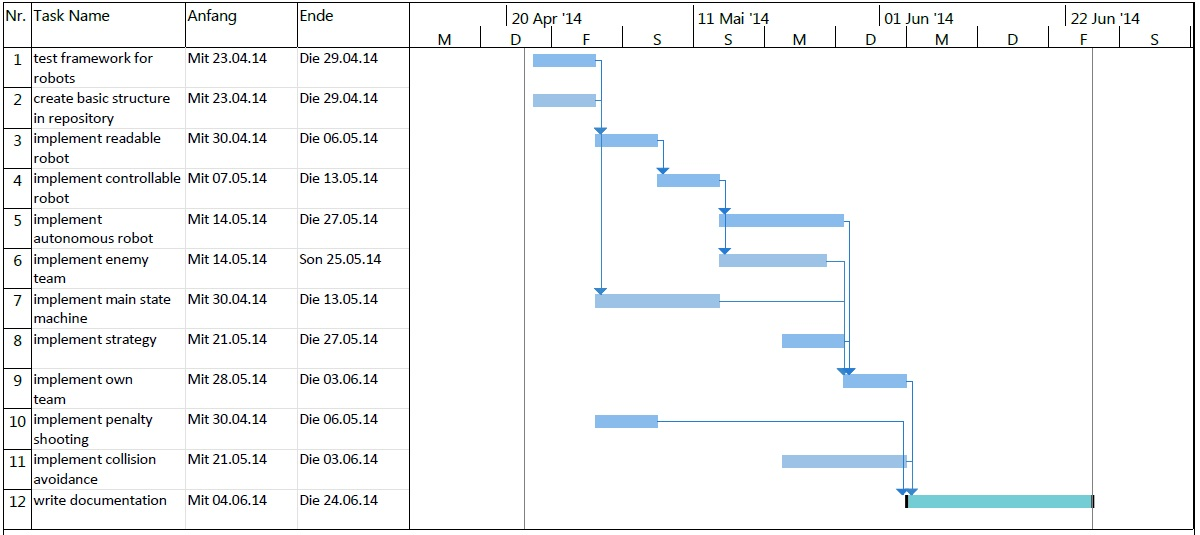
\includegraphics[width = 0.98\textwidth]{gantt_alt.jpg}
	\end{figure}
\end{frame}

\section{Implementation}
\subsection{Class Diagram}
\begin{frame}
	\frametitle{Layers}
	\begin{center}
		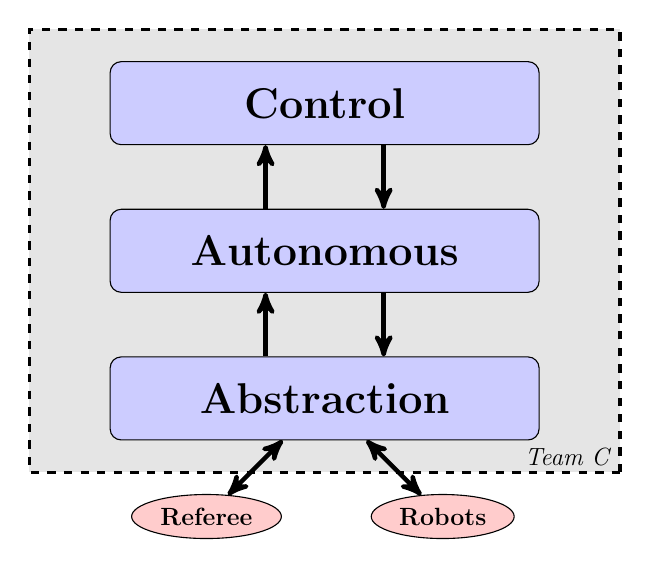
\begin{tikzpicture}[scale=0.75, transform shape]
			 Layers
			\node [block] (control) {\huge \textbf{Control}};
		    	\node [block, below of=control] (autonomous) {\huge \textbf{Autonomous}};
			\node [block, below of=autonomous] (abstraction) {\huge \textbf{Abstraction}};

			 Clouds
			\node [below of=abstraction, node distance=2cm] (babstraction) {} ;
			\node [cloud, right of=babstraction] (robots) {\large \textbf{Robots}};
			\node [cloud, left of=babstraction] (referee) {\large \textbf{Referee}};

			 Connections
			\path [line] ($(control.south) + (1,0)$) -- ($(autonomous.north) + (1,0)$);
			\path [line] ($(autonomous.north) + (-1,0)$) -- ($(control.south) + (-1,0)$);

			\path [line] ($(autonomous.south) + (1,0)$) -- ($(abstraction.north) + (1,0)$);
			\path [line] ($(abstraction.north) + (-1,0)$) -- ($(autonomous.south) + (-1,0)$);

			\path [dline] (referee) -- (abstraction);
			\path [dline] (robots) -- (abstraction);

			 Background Box
			\begin{pgfonlayer}{background}
				\draw [dashed, very thick, fill=black!10] ($(abstraction) +(5,-1.25)$) rectangle ($(control)+(-5,1.25)$);
				\draw ($(abstraction) +(5,-1)$) node [left] {\large \textit{Team C}};
			\end{pgfonlayer}
		\end{tikzpicture}
	\end{center}
\end{frame}

\begin{frame}
	\frametitle{Layers}
	\begin{center}
		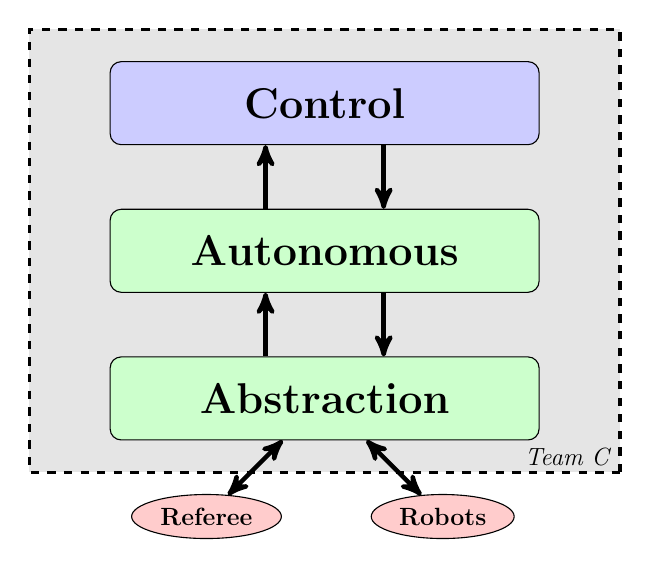
\begin{tikzpicture}[scale=0.75, transform shape]
		    	 Layers
			\node [block] (control) {\huge \textbf{Control}};
		    	\node [block-active, below of=control] (autonomous) {\huge \textbf{Autonomous}};
			\node [block-active, below of=autonomous] (abstraction) {\huge \textbf{Abstraction}};

			 Clouds
			\node [below of=abstraction, node distance=2cm] (babstraction) {} ;
			\node [cloud, right of=babstraction] (robots) {\large \textbf{Robots}};
			\node [cloud, left of=babstraction] (referee) {\large \textbf{Referee}};

			 Connections
			\path [line] ($(control.south) + (1,0)$) -- ($(autonomous.north) + (1,0)$);
			\path [line] ($(autonomous.north) + (-1,0)$) -- ($(control.south) + (-1,0)$);

			\path [line] ($(autonomous.south) + (1,0)$) -- ($(abstraction.north) + (1,0)$);
			\path [line] ($(abstraction.north) + (-1,0)$) -- ($(autonomous.south) + (-1,0)$);

			\path [dline] (referee) -- (abstraction);
			\path [dline] (robots) -- (abstraction);

			 Background Box
			\begin{pgfonlayer}{background}
				\draw [dashed, very thick, fill=black!10] ($(abstraction) +(5,-1.25)$) rectangle ($(control)+(-5,1.25)$);
				\draw ($(abstraction) +(5,-1)$) node [left] {\large \textit{Team C}};
			\end{pgfonlayer}
		\end{tikzpicture}
	\end{center}
\end{frame}

\begin{frame}
	\frametitle{Interface Autonomous - Abstraction}
	\begin{center}
		%!tikz editor 1.0
%!tikz source begin
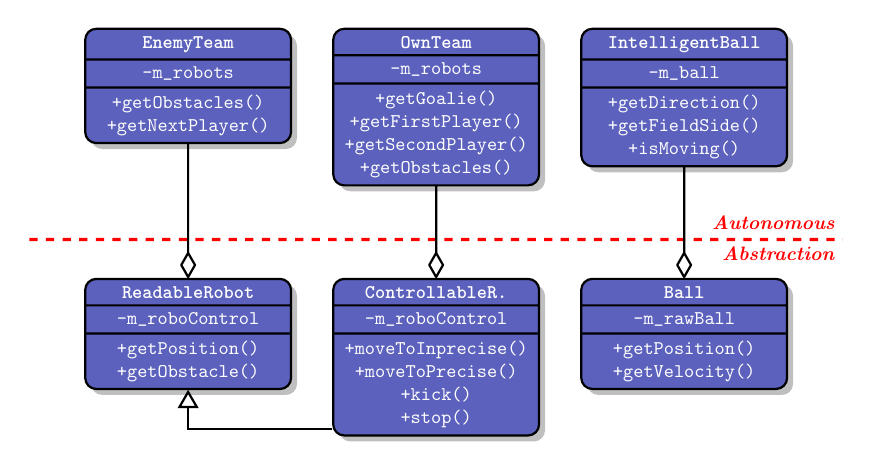
\begin{tikzpicture}[node distance=4.5cm, scale=0.7, transform shape]
	\font\btt=rm-lmtk10
	\definecolor{PresiBlue}{RGB}{50,57,171}
	
	\tikzstyle{class}=[
		rectangle, draw=black, rounded corners, rectangle split, rectangle split parts=3, 
		fill=PresiBlue!80, drop shadow, font=\tt,
        text centered, anchor=north, text=white, text width=3.5cm, thick]
		
	\tikzstyle{inheritance}=[draw, ->, >=open triangle 60, thick]
	\tikzstyle{property}=[draw, <-, >=open diamond, thick]
	\tikzstyle{line}=[-, thick]
   
   % Classes
      
	\node (enemyteam) [class]
	{
		\btt EnemyTeam
		
		\nodepart{second}
		-m\char`_robots
		
		\nodepart{third}
		+getObstacles()\\
		+getNextPlayer()
	};
	
	\node (ownteam) [class, right= of enemyteam.north , anchor=north]
	{
		\btt OwnTeam
		
		\nodepart{second}
		-m\char`_robots
		
		\nodepart{third}
		+getGoalie()\\
		+getFirstPlayer()\\
		+getSecondPlayer()\\
		+getObstacles()
	};
    
	\node (intelligentball) [class, right= of ownteam.north, anchor=north]
	{
		\btt IntelligentBall
		
		\nodepart{second}
		-m\char`_ball
		
		\nodepart{third}
		+getDirection()\\
		+getFieldSide()\\
		+isMoving()
	};
	
	\node (readablerobot) [class, below of=enemyteam]
	{
		\btt ReadableRobot
		
		\nodepart{second}
		-m\char`_roboControl
		
		\nodepart{third}
		+getPosition()\\
		+getObstacle()
	};
		
	\node (controllablerobot) [class, right= of readablerobot.north, anchor=north]
	{
		\btt ControllableR.
		
		\nodepart{second}
		-m\char`_roboControl
		
		\nodepart{third}
		+moveToInprecise()\\
		+moveToPrecise()\\
		+kick()\\
		+stop()
	};
	
	\node (ball) [class, right= of controllablerobot.north, anchor=north]
	{
		\btt Ball
		
		\nodepart{second}
		-m\char`_rawBall
		
		\nodepart{third}
		+getPosition()\\
		+getVelocity()
	};
	
	% Connections
	\path [inheritance] (controllablerobot.west) +(0,-1.3) -| (readablerobot);
	\path [property] (controllablerobot) -- (ownteam);
	\path [property] (readablerobot) -- (enemyteam);
	\path [property] (ball) -- (intelligentball);
	
	% Background Box
	\begin{pgfonlayer}{background}
		\draw [dashed, very thick, red] ($(readablerobot.north west) + (-1,0.7)$) -- ($(ball.north east) + (1,0.7)$);
		\draw ($(ball.north east) + (1,0.45)$) node [left, red] {\textbf{\textit{Abstraction}}};
		\draw ($(ball.north east) + (1,1)$) node [left, red] {\textbf{\textit{Autonomous}}};
	\end{pgfonlayer}

	
\end{tikzpicture}
%!tikz source end

	\end{center}
\end{frame}

\begin{frame}
	\frametitle{Layers}
	\begin{center}
		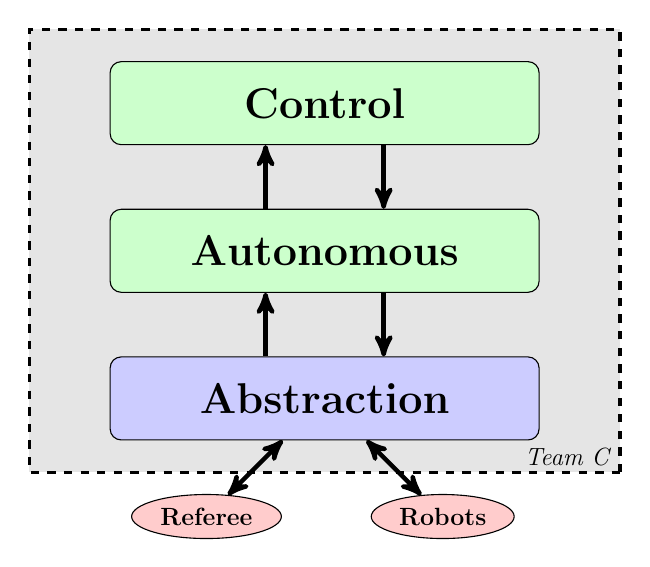
\begin{tikzpicture}[scale=0.75, transform shape]
		    	 Layers
			\node [block-active] (control) {\huge \textbf{Control}};
		    	\node [block-active, below of=control] (autonomous) {\huge \textbf{Autonomous}};
			\node [block, below of=autonomous] (abstraction) {\huge \textbf{Abstraction}};

			 Clouds
			\node [below of=abstraction, node distance=2cm] (babstraction) {} ;
			\node [cloud, right of=babstraction] (robots) {\large \textbf{Robots}};
			\node [cloud, left of=babstraction] (referee) {\large \textbf{Referee}};

			 Connections
			\path [line] ($(control.south) + (1,0)$) -- ($(autonomous.north) + (1,0)$);
			\path [line] ($(autonomous.north) + (-1,0)$) -- ($(control.south) + (-1,0)$);

			\path [line] ($(autonomous.south) + (1,0)$) -- ($(abstraction.north) + (1,0)$);
			\path [line] ($(abstraction.north) + (-1,0)$) -- ($(autonomous.south) + (-1,0)$);

			\path [dline] (referee) -- (abstraction);
			\path [dline] (robots) -- (abstraction);

			 Background Box
			\begin{pgfonlayer}{background}
				\draw [dashed, very thick, fill=black!10] ($(abstraction) +(5,-1.25)$) rectangle ($(control)+(-5,1.25)$);
				\draw ($(abstraction) +(5,-1)$) node [left] {\large \textit{Team C}};
			\end{pgfonlayer}
		\end{tikzpicture}
	\end{center}
\end{frame}

\begin{frame}
	\frametitle{Interface Control - Autonomous}
	\center
	%!tikz editor 1.0
%!tikz source begin
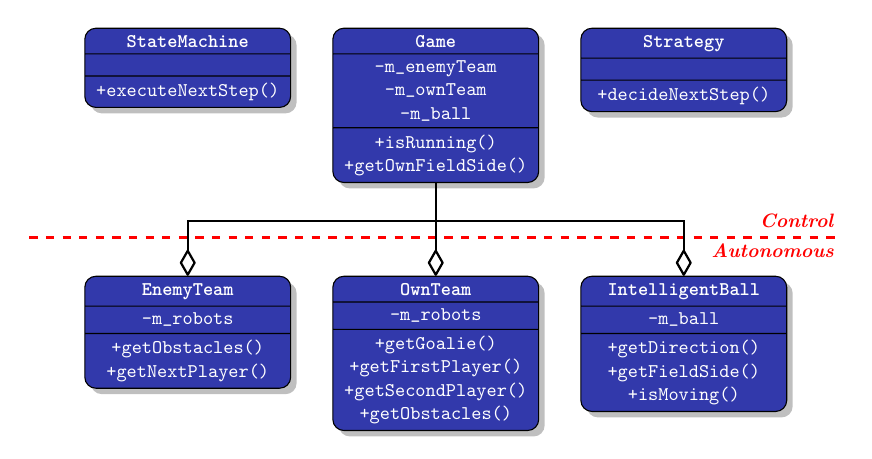
\begin{tikzpicture}[node distance=4.5cm, scale=0.7, transform shape]
	\font\btt=rm-lmtk10
	\definecolor{PresiBlue}{RGB}{50,57,171}
	
	\tikzstyle{class}=[
		rectangle, draw=black, rounded corners, rectangle split, rectangle split parts=3, 
		fill=PresiBlue, drop shadow, font=\tt,
        text centered, anchor=north, text=white, text width=3.5cm]
		
	\tikzstyle{comment}=[
		rectangle, draw=black, rounded corners, fill=green, drop shadow,
        text centered, anchor=north, text=white, text width=3cm]
		
	\tikzstyle{inheritance}=[draw, ->, >=open triangle 60, thick]
	\tikzstyle{property}=[draw, <-, >=open diamond, thick]
	\tikzstyle{line}=[-, thick]
   
   % Classes
      
	\node (enemyteam) [class]
	{
		\btt EnemyTeam
		
		\nodepart{second}
		-m\char`_robots
		
		\nodepart{third}
		+getObstacles()\\
		+getNextPlayer()
	};
	
	\node (ownteam) [class, right= of enemyteam.north , anchor=north]
	{
		\btt OwnTeam
		
		\nodepart{second}
		-m\char`_robots
		
		\nodepart{third}
		+getGoalie()\\
		+getFirstPlayer()\\
		+getSecondPlayer()\\
		+getObstacles()
	};
    
	\node (intelligentball) [class, right= of ownteam.north, anchor=north]
	{
		\btt IntelligentBall
		
		\nodepart{second}
		-m\char`_ball
		
		\nodepart{third}
		+getDirection()\\
		+getFieldSide()\\
		+isMoving()
	};
	
	\node (game) [class, above= of ownteam, anchor=north]
	{
		\btt Game
		
		\nodepart{second}
		-m\char`_enemyTeam\\
		-m\char`_ownTeam\\
		-m\char`_ball\\
		
		\nodepart{third}
		+isRunning()\\
		+getOwnFieldSide()
	};
	
	\node (statemachine) [class, left= of game.north, anchor=north]
	{
		\btt StateMachine
		
		\nodepart{third}
		+executeNextStep()
	};
	
	\node (strategy) [class, right= of game.north, anchor=north]
	{
		\btt Strategy
		
		\nodepart{third}
		+decideNextStep()
	};
	% Connections
	\path [property] (enemyteam.north) -- +(0,1) -| (game.south);
	\path [property] (ownteam.north) -- +(0,1) -| (game.south);
	\path [property] (intelligentball.north) -- +(0,1) -| (game.south);
	
	% Background Box
	\begin{pgfonlayer}{background}
		\draw [dashed, very thick, red] ($(enemyteam.north west) + (-1,0.7)$) -- ($(intelligentball.north east) + (1,0.7)$);
		\draw ($(intelligentball.north east) + (1,0.45)$) node [left, red] {\textbf{\textit{Autonomous}}};
		\draw ($(intelligentball.north east) + (1,1)$) node [left, red] {\textbf{\textit{Control}}};
	\end{pgfonlayer}

	
\end{tikzpicture}
%!tikz source end

\end{frame}

\begin{frame}
	\frametitle{Main Application}
	\center
	\begin{figure}
		\centering
		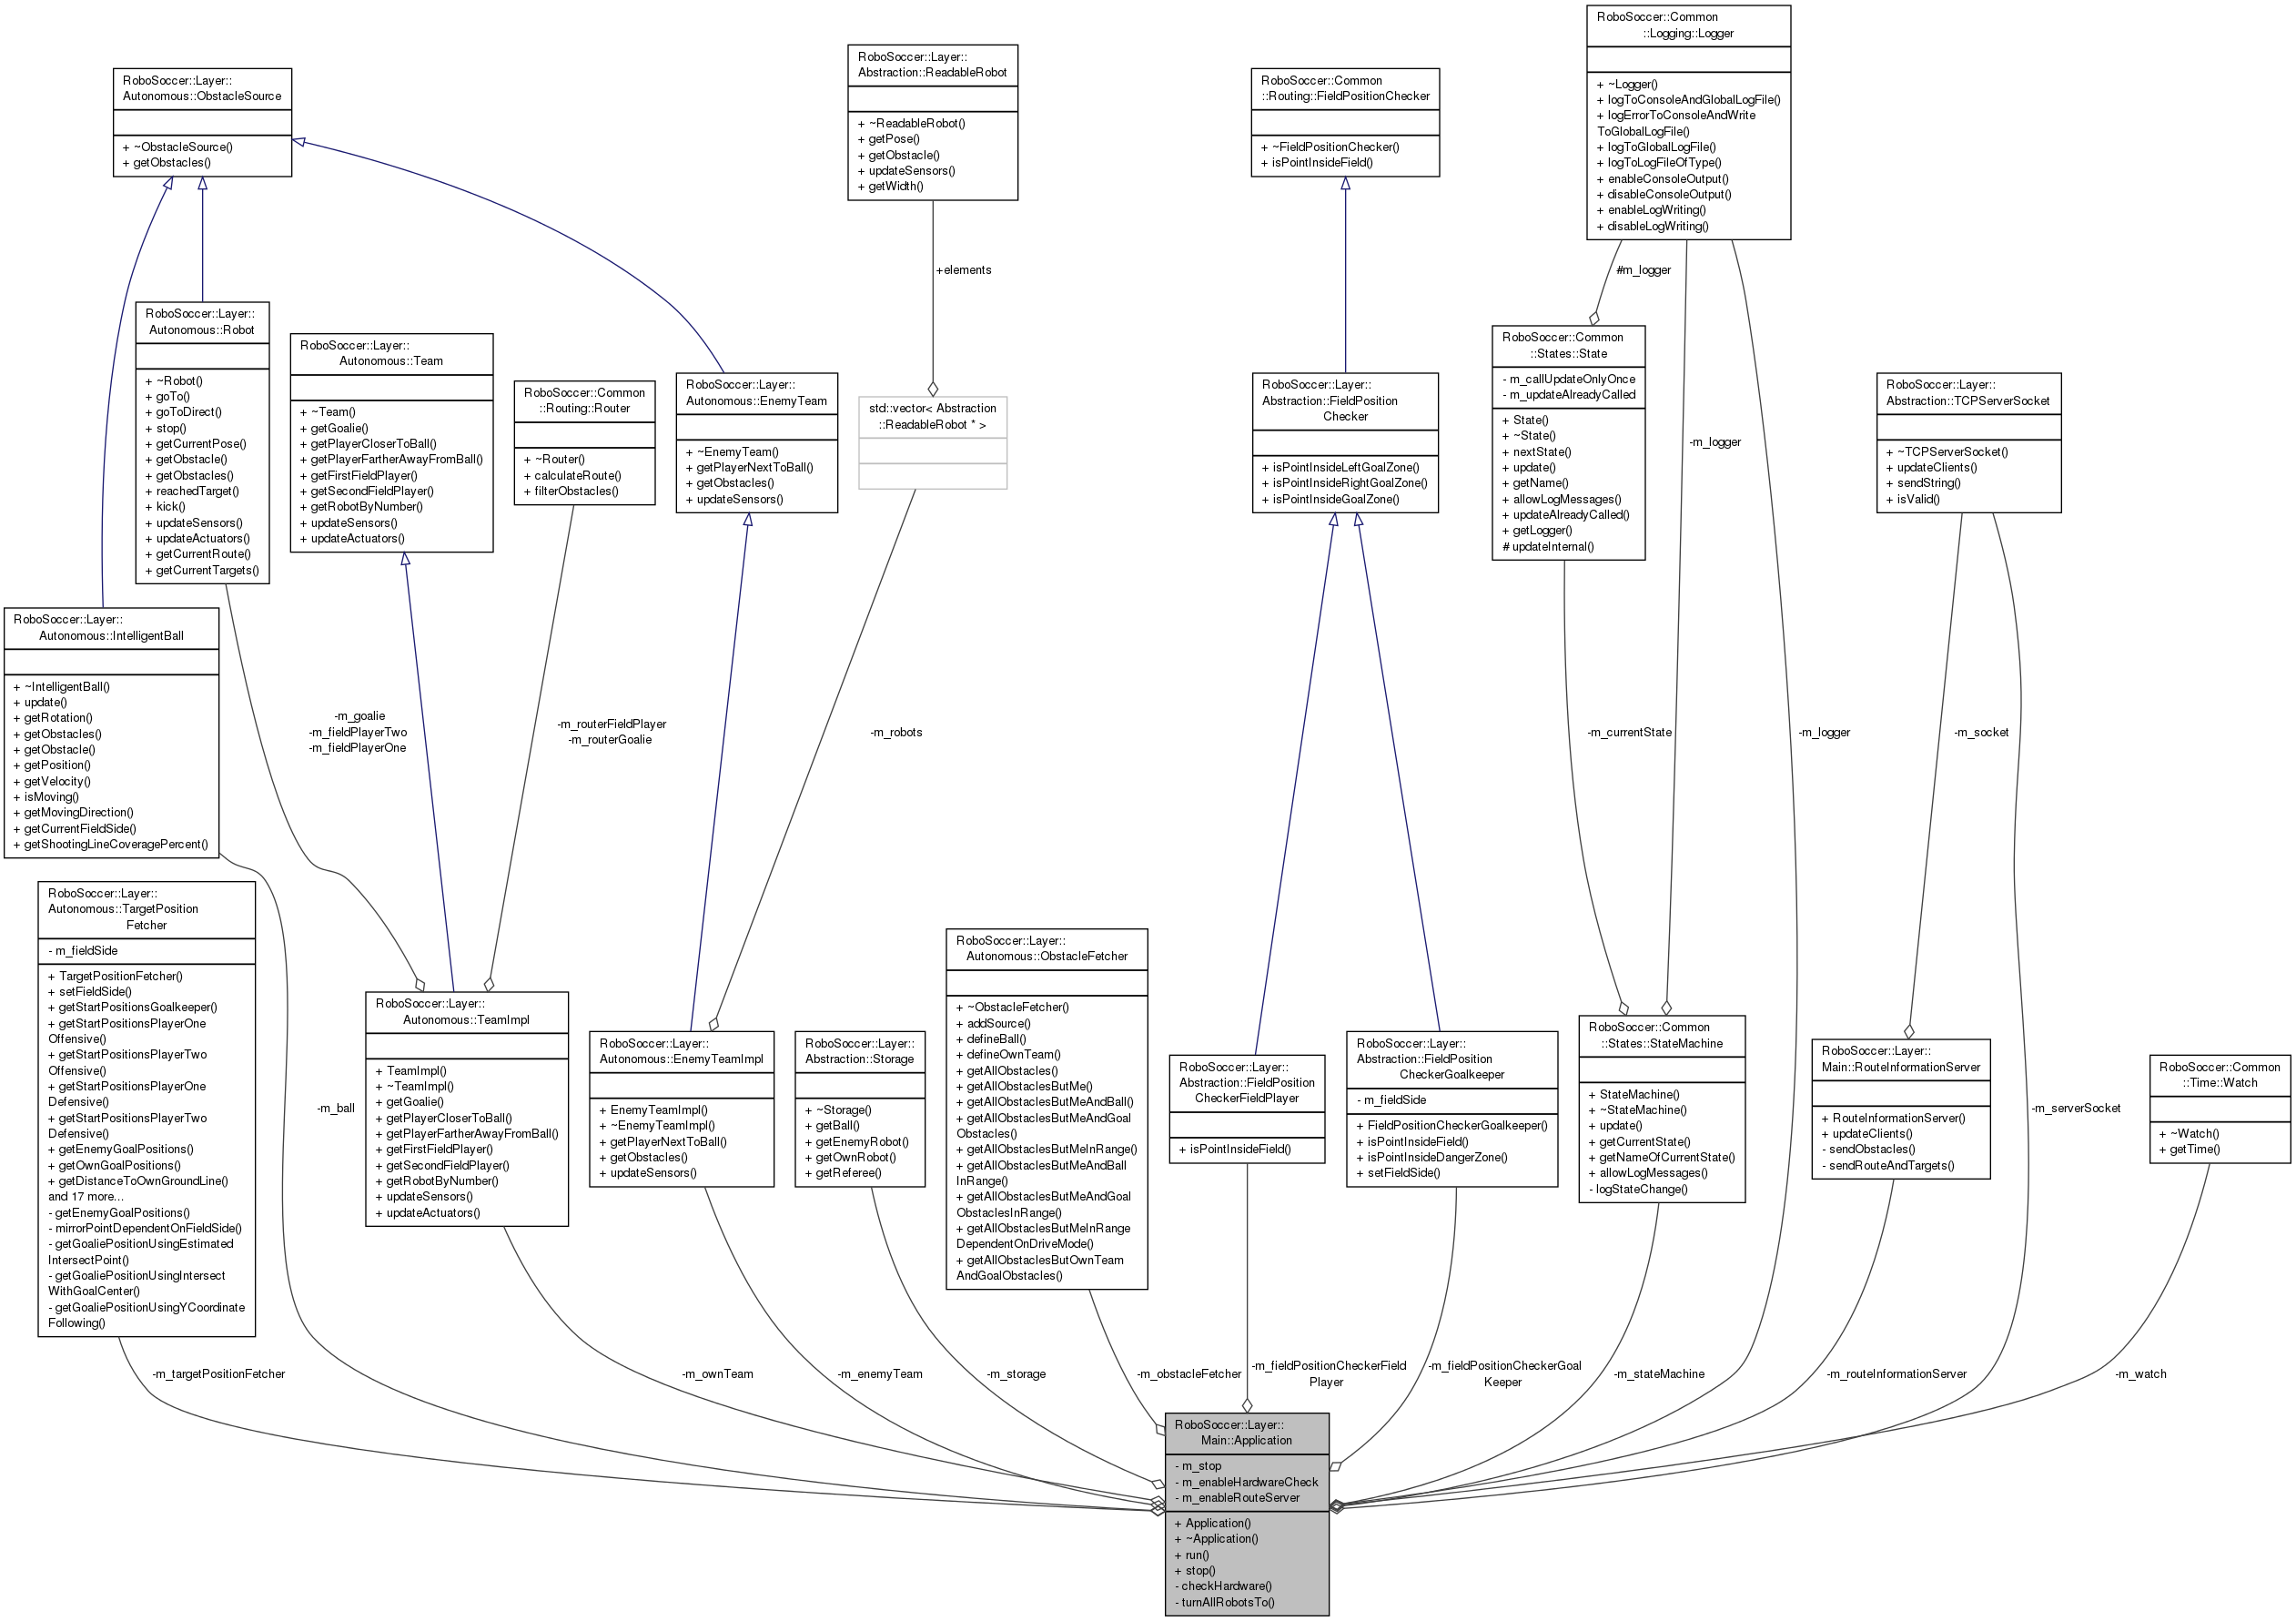
\includegraphics[width = \textwidth]{collaboration_graph_application.png}
	\end{figure}
\end{frame}

\begin{frame}
	\frametitle{Main Application}
	\center
	\begin{figure}
		\centering
		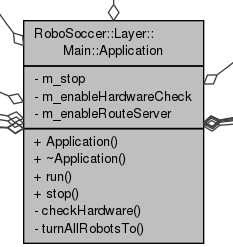
\includegraphics[width = \textwidth]{collaboration_graph_application_zoomed.png}
	\end{figure}
\end{frame}

\begin{frame}
	\frametitle{States}
	\center
	\begin{figure}
		\centering
		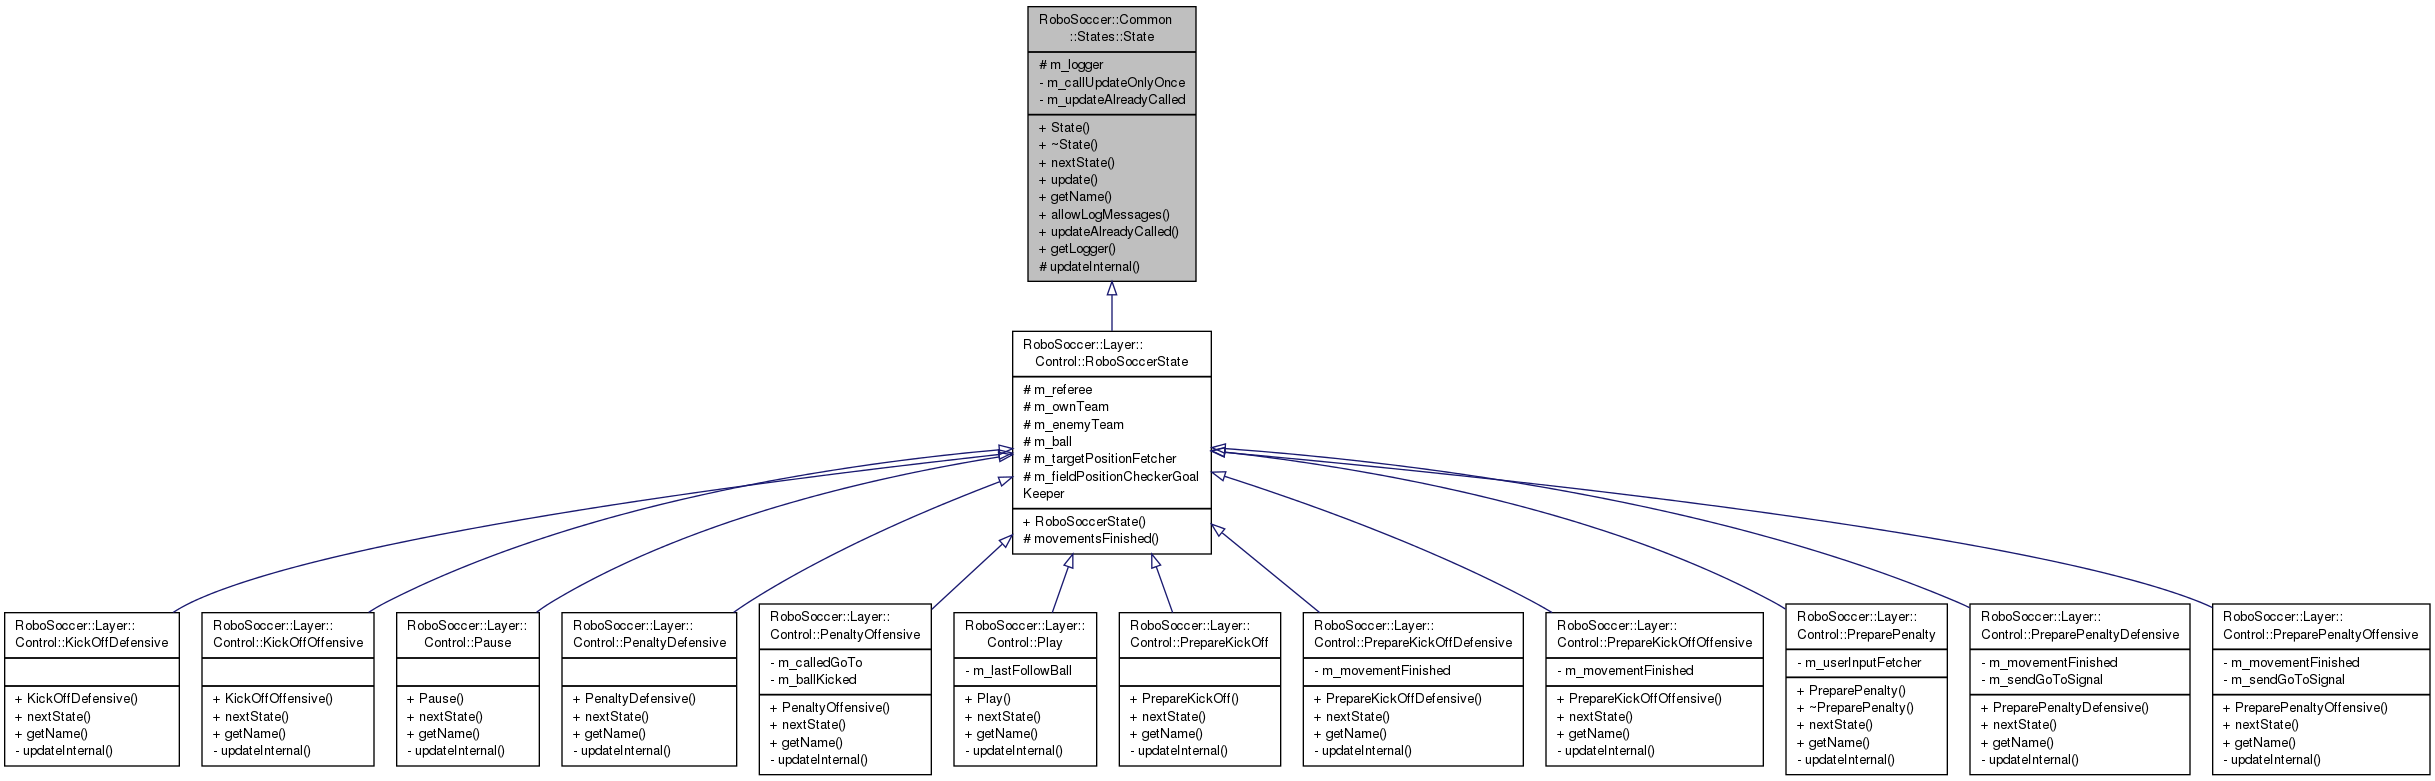
\includegraphics[width = \textwidth]{inheritance_graph_states.png}
	\end{figure}
\end{frame}

\begin{frame}
	\frametitle{States}
	\center
	\begin{figure}
		\centering
		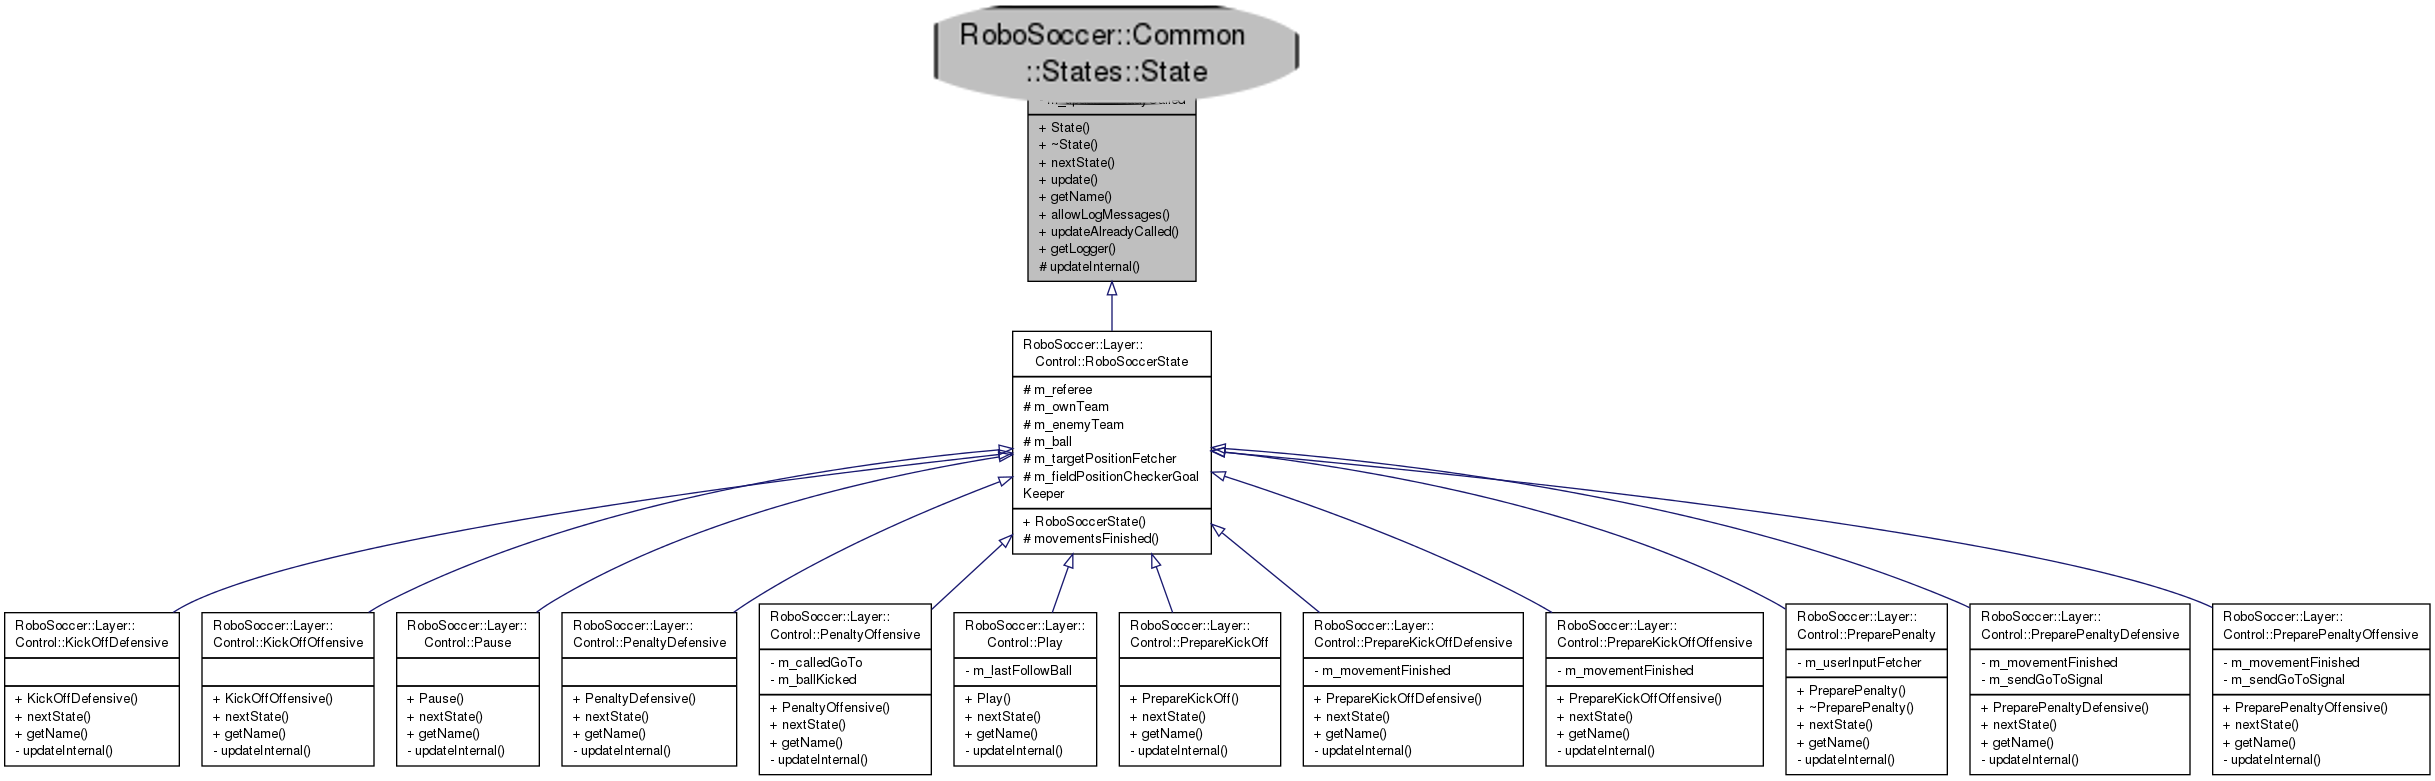
\includegraphics[width = \textwidth]{inheritance_graph_states_zoomed.png}
	\end{figure}
\end{frame}

\begin{frame}
	\frametitle{State Machine}
	\fontsize{6pt}{7.2}\selectfont
	\begin{center}
		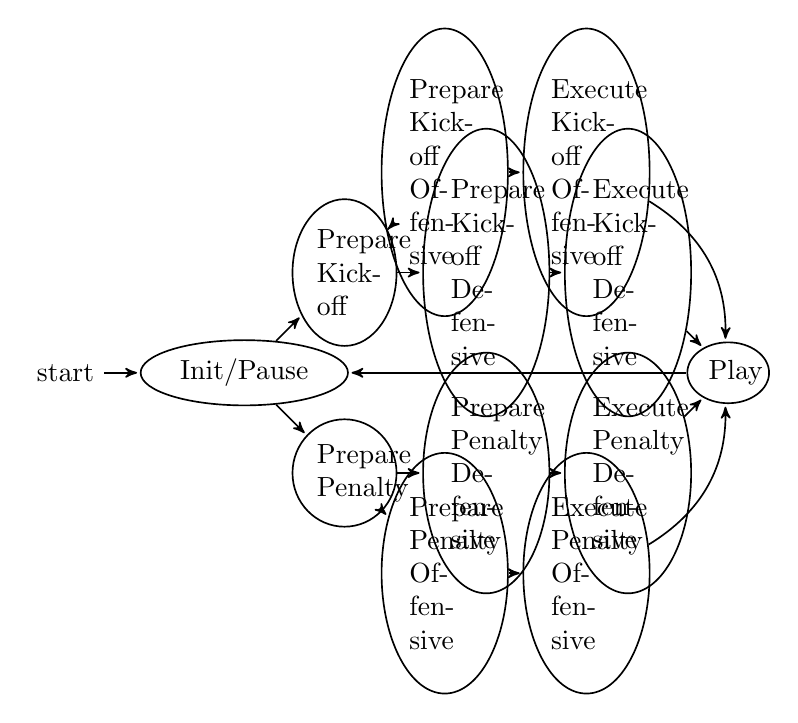
\begin{tikzpicture}[->,>=stealth',shorten >=1pt,auto,node distance=1.8cm,semithick]
			\tikzstyle{every state}=[draw=none,text=black]
			\tikzset{elliptic state/.style={draw,ellipse}}

			\node[initial,elliptic state] (init)                    {Init/Pause};
			\node[elliptic state]         (prepareKickOff) [above right of=init,text width=0.7cm] {Prepare Kickoff};
			\node[elliptic state]         (prepareKickOffOffensive) [above right of=prepareKickOff,text width=0.9cm] {Prepare Kickoff Offensive};
			\node[elliptic state]         (executeKickOffOffensive) [right of=prepareKickOffOffensive,text width=0.9cm] {Execute Kickoff Offensive};
			\node[elliptic state]         (prepareKickOffDefensive) [right of=prepareKickOff,text width=0.9cm]       {Prepare Kickoff Defensive};
			\node[elliptic state]         (executeKickOffDefensive) [right of=prepareKickOffDefensive,text width=0.9cm]       {Execute Kickoff Defensive};
			\node[elliptic state]         (preparePenalty) [below right of=init,text width=0.7cm] {Prepare Penalty};
			\node[elliptic state]         (preparePenaltyOffensive) [below right of=preparePenalty,text width=0.9cm] {Prepare Penalty Offensive};
			\node[elliptic state]         (executePenaltyOffensive) [right of=preparePenaltyOffensive,text width=0.9cm] {Execute Penalty Offensive};
			\node[elliptic state]         (preparePenaltyDefensive) [right of=preparePenalty,text width=0.9cm]       {Prepare Penalty Defensive};
			\node[elliptic state]         (executePenaltyDefensive) [right of=preparePenaltyDefensive,text width=0.9cm]       {Execute Penalty Defensive};
			\node[elliptic state]         (play) [below right of=executeKickOffDefensive,text width=0.5cm]       {Play};

			\path (init)
						edge (prepareKickOff)
			  			edge (preparePenalty)
			      (prepareKickOff)
			        	edge (prepareKickOffOffensive)
			            edge (prepareKickOffDefensive)
			      (prepareKickOffOffensive)
			        	edge (executeKickOffOffensive)
			      (prepareKickOffDefensive)
			        	edge (executeKickOffDefensive)
			      (executeKickOffOffensive)
				       	edge [bend left] (play)
			      (executeKickOffDefensive)
			        	edge (play)
			      (preparePenalty)
			        	edge (preparePenaltyOffensive)
			            edge (preparePenaltyDefensive)
			      (preparePenaltyOffensive)
			        	edge (executePenaltyOffensive)
			      (preparePenaltyDefensive)
			        	edge (executePenaltyDefensive)
			      (executePenaltyOffensive)
			        	edge [bend right] (play)
			      (executePenaltyDefensive)
			        	edge (play)
			      (play)
			        	edge (init);
		\end{tikzpicture}
	\end{center}
\end{frame}

\begin{frame}
	\frametitle{Robot States}
	\center
	\begin{figure}
		\centering
		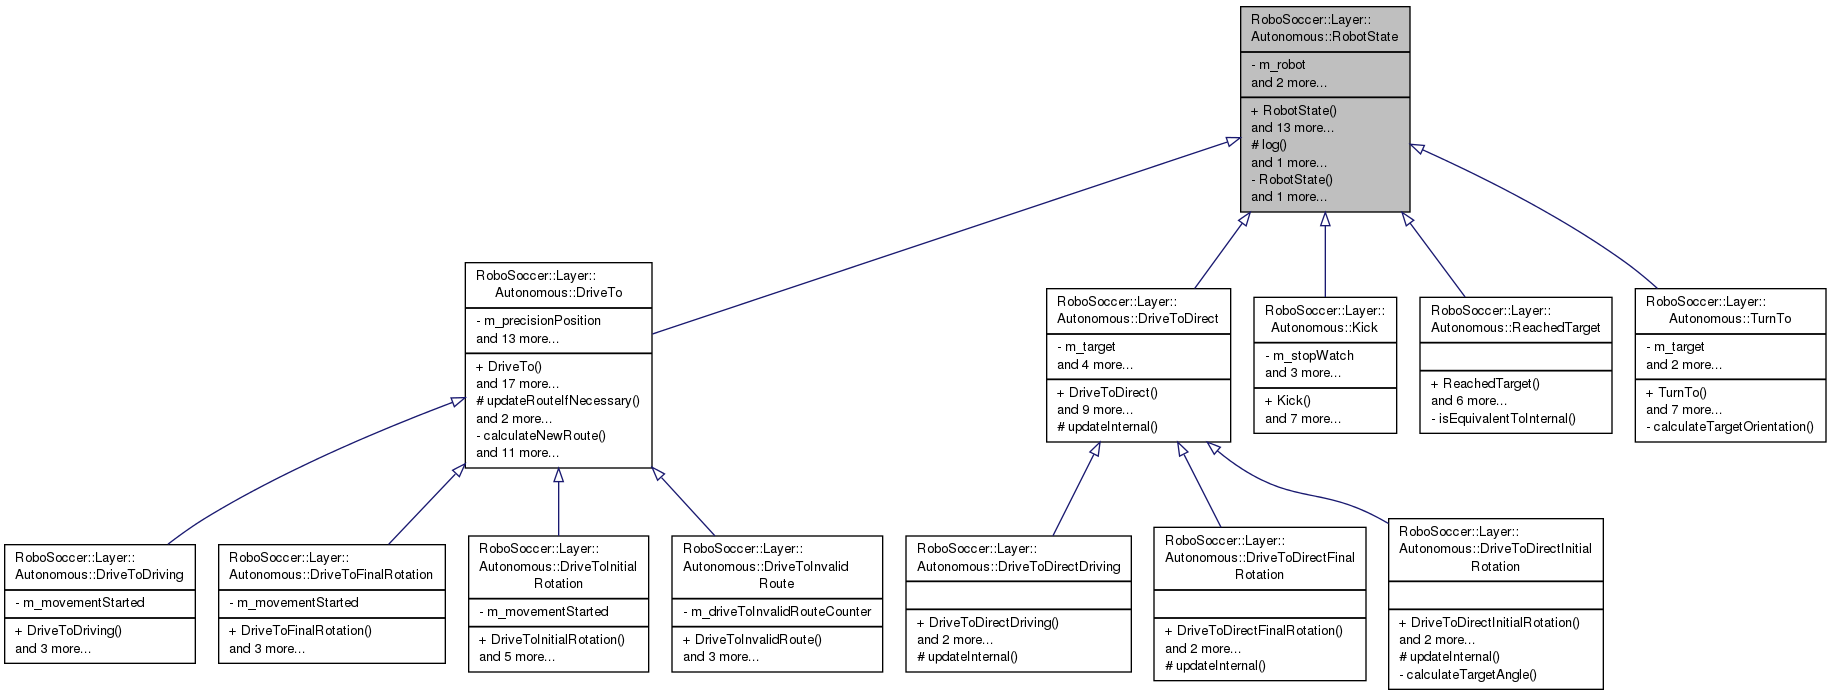
\includegraphics[width = \textwidth]{inheritance_graph_robotstates.png}
	\end{figure}
\end{frame}

\begin{frame}
	\frametitle{Robot States}
	\center
	\begin{figure}
		\centering
		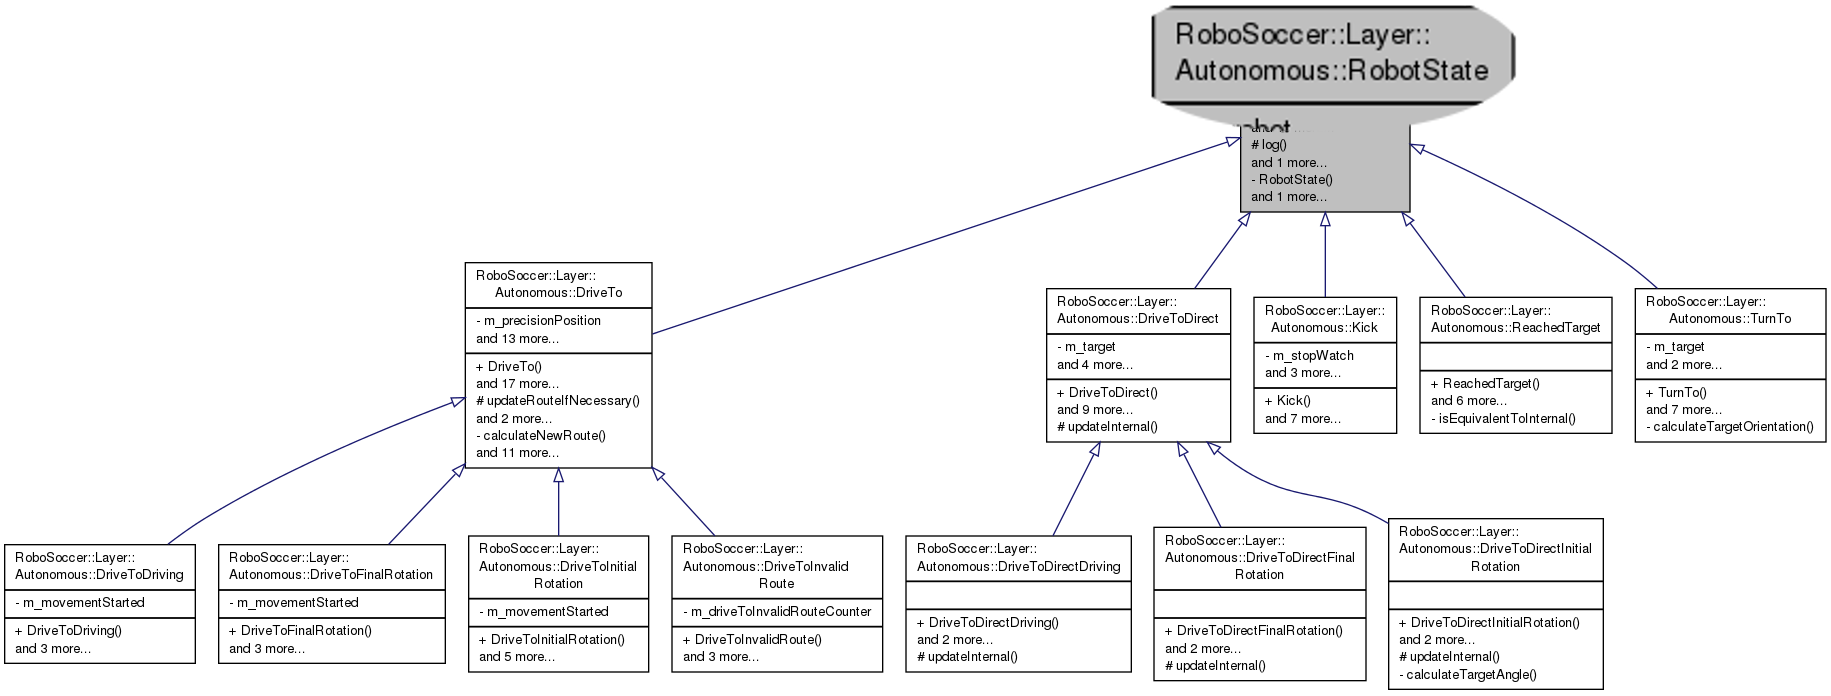
\includegraphics[width = \textwidth]{inheritance_graph_robotstates_zoomed.png}
	\end{figure}
\end{frame}

\begin{frame}
	\frametitle{DriveTo}
	\center
	\begin{figure}
		\centering
		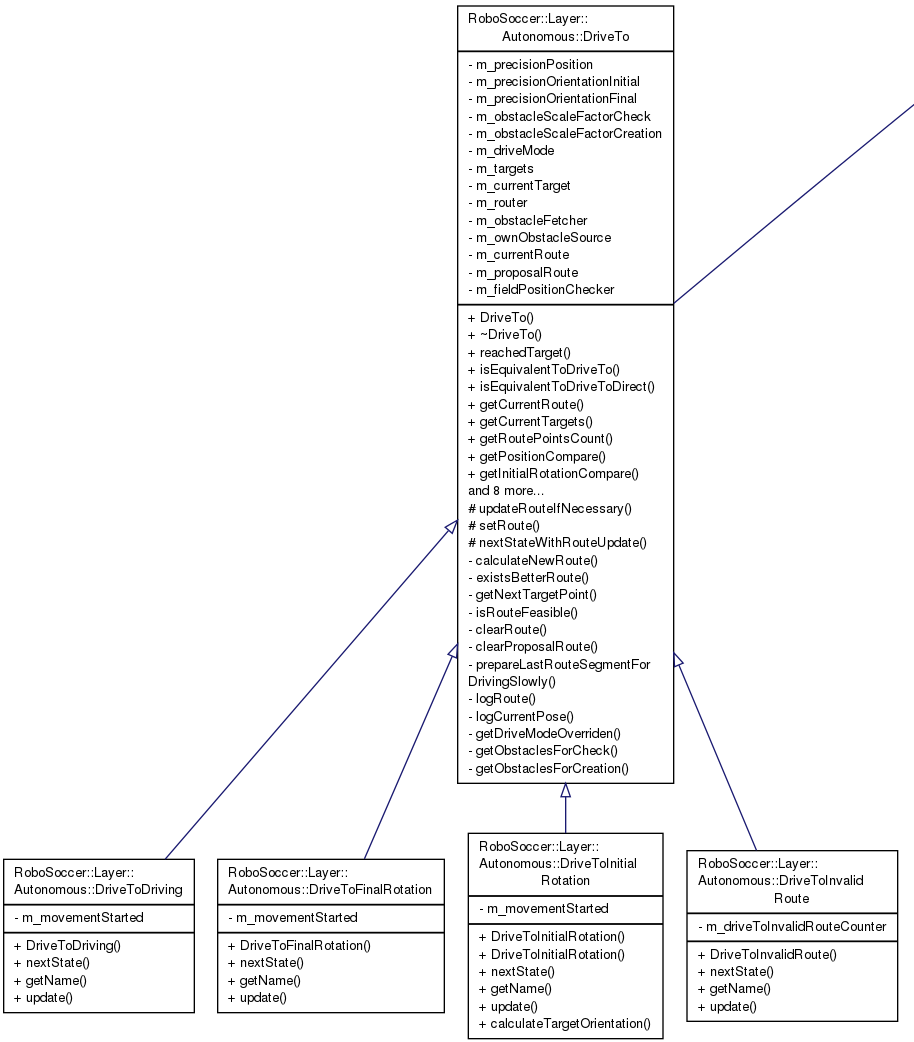
\includegraphics[width = \textwidth]{inheritance_graph_robotstates_driveto.png}
	\end{figure}
\end{frame}

\begin{frame}
	\frametitle{Robot States}
	\center
	\begin{figure}
		\centering
		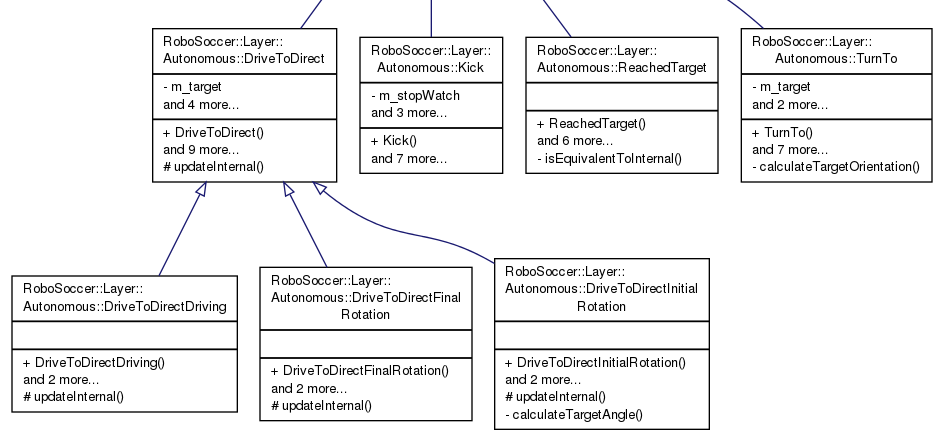
\includegraphics[width = \textwidth]{inheritance_graph_robotstates_rest.png}
	\end{figure}
\end{frame}

\begin{frame}
	\frametitle{Tree Nodes}
	\center
	\begin{figure}
		\centering
		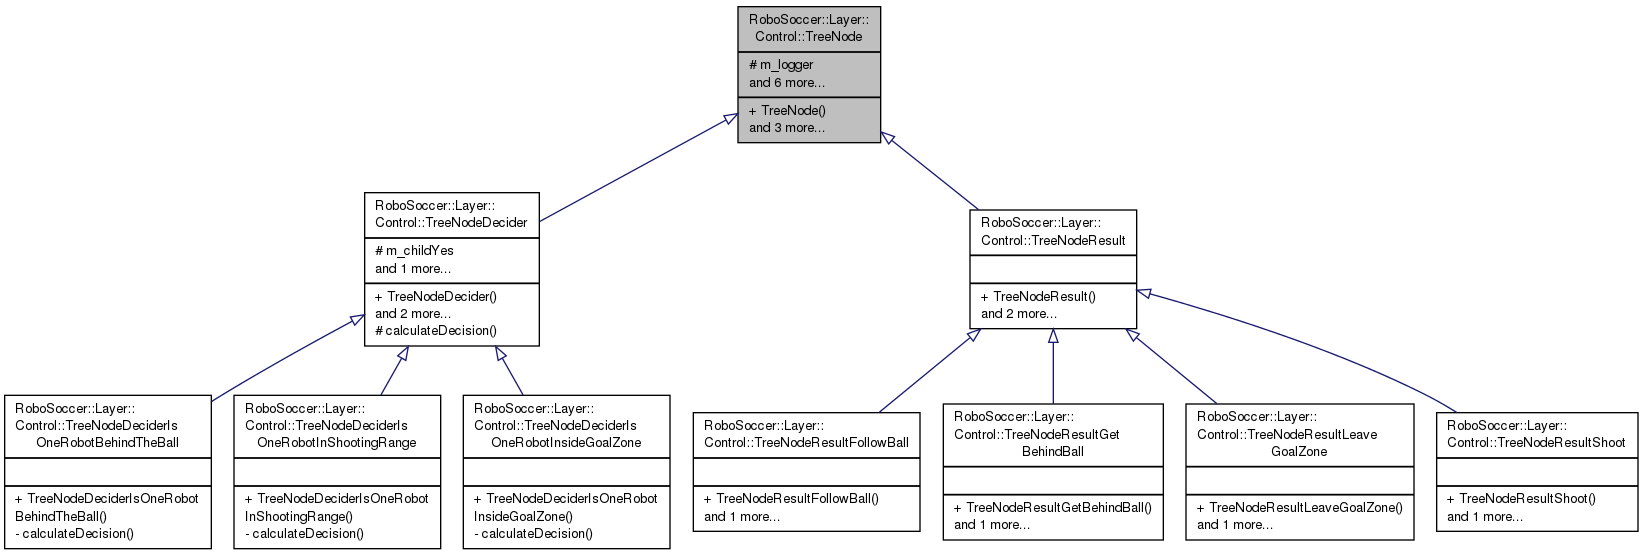
\includegraphics[width = \textwidth]{inheritance_graph_treenode.png}
	\end{figure}
\end{frame}

\begin{frame}
	\frametitle{Tree Nodes}
	\center
	\begin{figure}
		\centering
		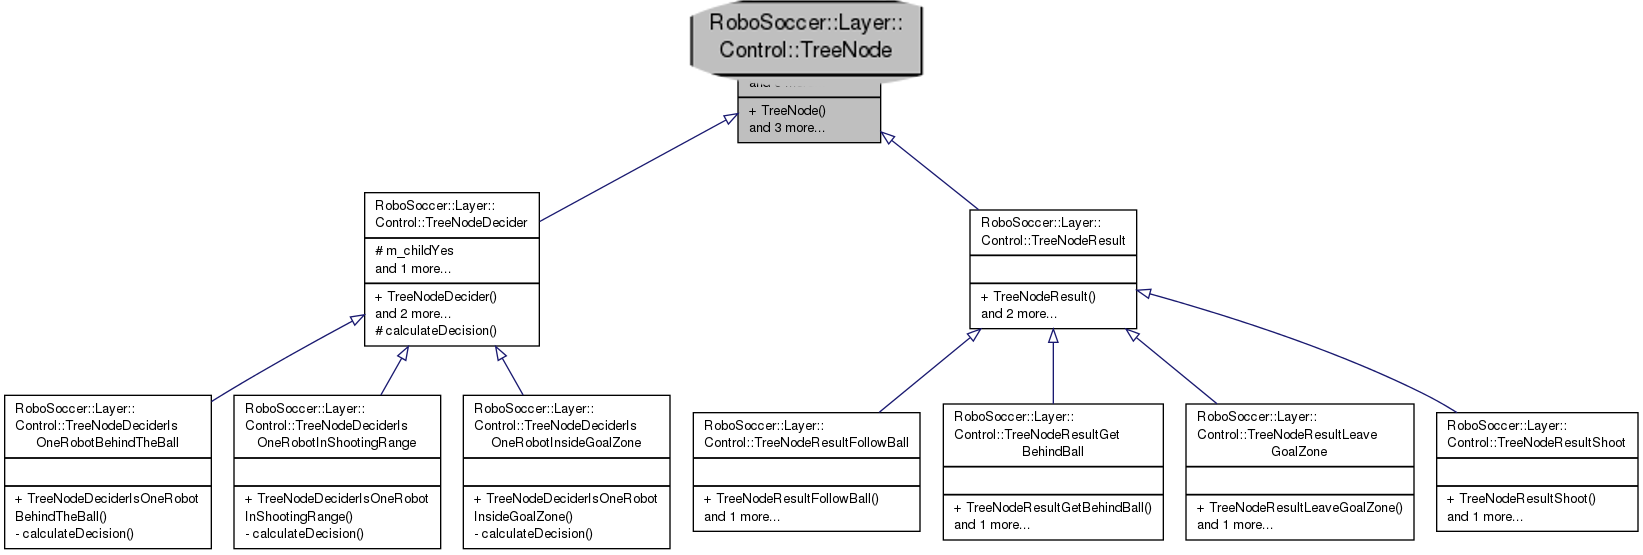
\includegraphics[width = \textwidth]{inheritance_graph_treenode_zoomed.png}
	\end{figure}
\end{frame}

\begin{frame}
	\frametitle{Tree Node Deciders}
	\center
	\begin{figure}
		\centering
		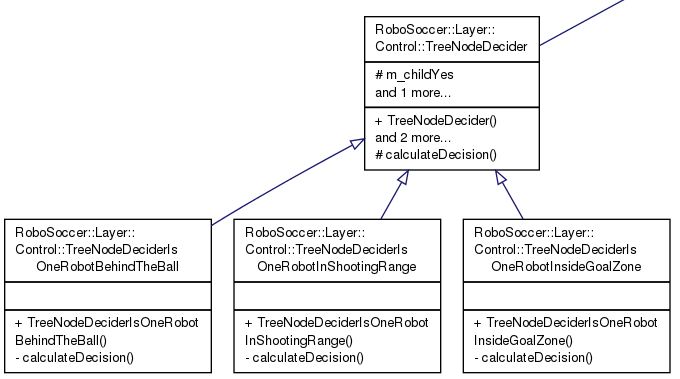
\includegraphics[width = 0.8\textwidth]{inheritance_graph_treenode_deciders.png}
	\end{figure}
\end{frame}

\begin{frame}
	\frametitle{Tree Node Results}
	\center
	\begin{figure}
		\centering
		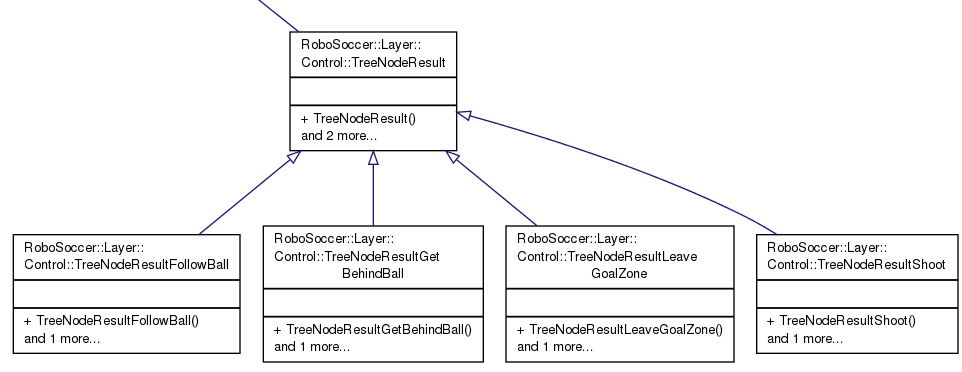
\includegraphics[width = \textwidth]{inheritance_graph_treenode_results.png}
	\end{figure}
\end{frame}

\subsection{Collision Avoidance}
\begin{frame}
	\frametitle{Collision Avoidance}
	\begin{center}
		\resizebox{!}{0.8\textheight}{
			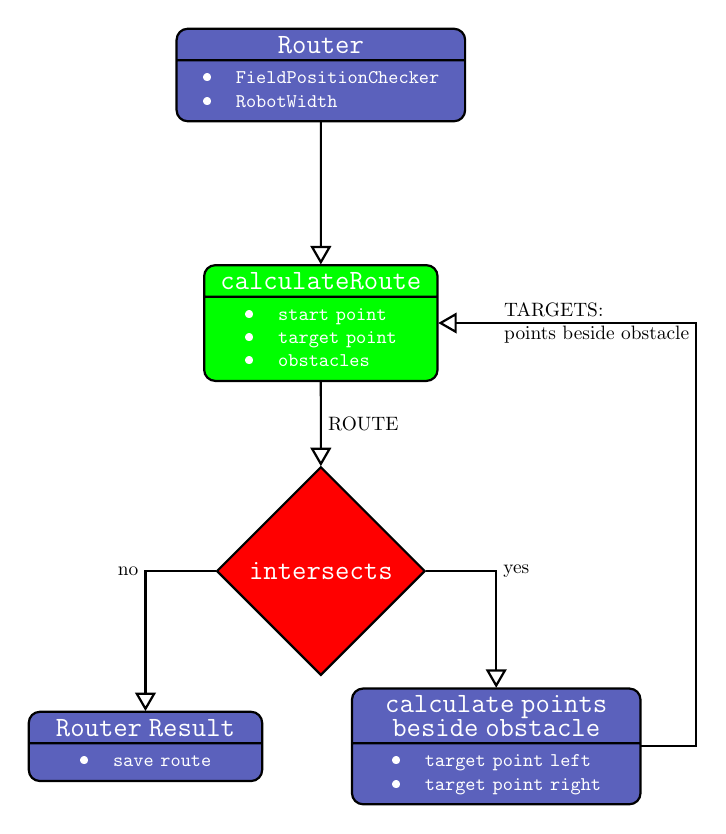
\begin{tikzpicture}[node distance=4.5cm, scale=0.7, transform shape]
	\font\btt=rm-lmtk10
	\definecolor{PresiBlue}{RGB}{50,57,171}
	
	\tikzstyle{class}=[
		rectangle, draw=black, rounded corners, rectangle split, rectangle split parts=2, 
		fill=PresiBlue!80, font=\tt,
        text centered, anchor=north, text=white, text width=5cm, thick]
        
       \tikzstyle{call}=[
		rectangle, draw=black, rounded corners, rectangle split, rectangle split parts=2, 
		fill=green, font=\tt,
        text centered, anchor=north, text=white, text width=4cm, thick]
        
	\tikzstyle{decision} = [
		diamond, draw=black, fill=red, font=\tt,
        text centered, anchor=north, text=white, text width=3cm, thick]
		
	\tikzstyle{arrow}=[draw, ->, >=open triangle 60, thick]
	\tikzstyle{property}=[draw, <-, >=open diamond, thick]
	\tikzstyle{line}=[-, thick]
	
	\node (constructor) [class]
	{
		{\Large \texttt{\textbf{Router}}}
		
		\nodepart{second}
		\begin{tabular}{ll}
			\textbullet & FieldPositionChecker\\
			\textbullet & RobotWidth
		\end{tabular}
	};
	
	\node (calculate) [call,below of=constructor]
	{
		{\Large \texttt{\textbf{calculateRoute}}}
		
		\nodepart{second}
		\begin{tabular}{ll}
			\textbullet & start point\\
			\textbullet & target point\\
			\textbullet & obstacles
		\end{tabular}
	};
	
	\node (intersects) [decision,below of=calculate]
	{
		{\Large \texttt{\textbf{intersects}}}
	};
	
	\node (finish) [class, below left of=intersects,text width=4cm]
	{
		{\Large \texttt{\textbf{Router Result}}}
		
		\nodepart{second}
		\begin{tabular}{ll}
			\textbullet & save route
		\end{tabular}
	};
	
	\node (beside) [class, below right of=intersects]
	{
		{\Large \texttt{\textbf{calculate points beside obstacle}}}
		
		\nodepart{second}
		\begin{tabular}{ll}
			\textbullet & target point left\\
			\textbullet & target point right
		\end{tabular}
	};
	
	\path[arrow] (constructor) -- (calculate);
	\path[arrow] (calculate) -- (intersects) node [midway,right] {ROUTE};
	\path[arrow] (intersects) -| (finish) node [midway,left] {no};
	\path[arrow] (intersects) -| (beside) node [midway,right] {yes};
	\path[arrow] (beside.east) -- ++(1,0) |- (calculate) node [pos=0.5, left,align=left] {TARGETS: \\ points beside obstacle};
	
\end{tikzpicture}
		}
	\end{center}
\end{frame}

\begin{frame}
	\frametitle{Router}
	\begin{center}
		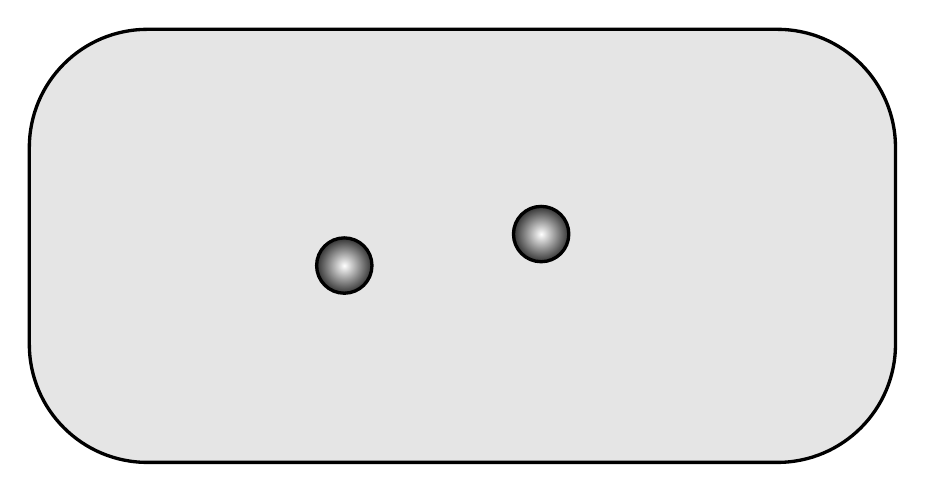
\begin{tikzpicture}
			 Background Box
			\begin{pgfonlayer}{background}
				\draw [rounded corners=1.5cm, very thick, fill=black!10] (-2.5,-3) rectangle (8.5,2.5);
			\end{pgfonlayer}
			 Folie 1
			\robot at (0,0) {};
			\node[obstacle] at (1.5,-.5) {};
			\node[obstacle] at (4,-0.1) {};
			\goal at (6,0) {};
		\end{tikzpicture}
	\end{center}
\end{frame}

\begin{frame}
	\frametitle{Router}
	\begin{center}
		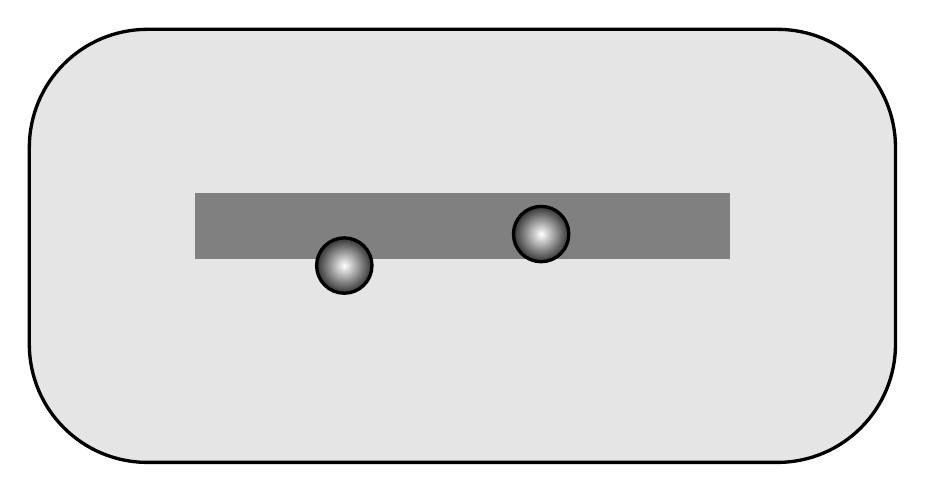
\begin{tikzpicture}
			 Background Box
			\begin{pgfonlayer}{background}
				\draw [rounded corners=1.5cm, very thick, fill=black!10] (-2.5,-3) rectangle (8.5,2.5);
			\end{pgfonlayer}
			 Folie 2
			\path[edge] (-0.4,0) -- (6.4,0);
			\robot at (0,0) {};
			\node[obstacle] at (1.5,-.5) {};
			\node[obstacle] at (4,-0.1) {};
			\goal at (6,0) {};
		\end{tikzpicture}
	\end{center}
\end{frame}

\begin{frame}
	\frametitle{Router}
	\begin{center}
		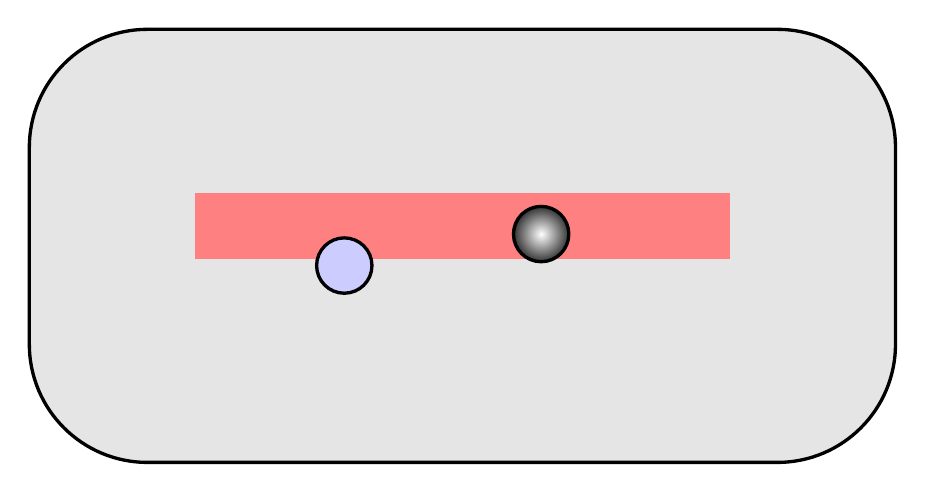
\begin{tikzpicture}
			 Background Box
			\begin{pgfonlayer}{background}
				\draw [rounded corners=1.5cm, very thick, fill=black!10] (-2.5,-3) rectangle (8.5,2.5);
			\end{pgfonlayer}
			 Folie 3
			\path[ignored edge] (-0.4,0) -- (6.4,0);
			\robot at (0,0) {};
			\node[selected obstacle] at (1.5,-.5) {};
			\node[obstacle] at (4,-0.1) {};
			\goal at (6,0) {};
			\goalHelp at (1.5,.5) {};
			\goalHelp at (1.5,-1.8) {};
		\end{tikzpicture}
	\end{center}
\end{frame}

\begin{frame}
	\frametitle{Router}
	\begin{center}
		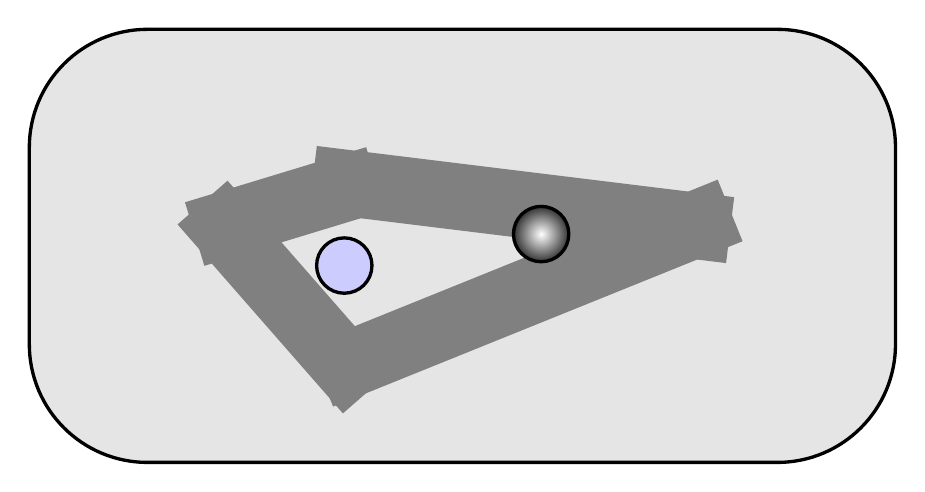
\begin{tikzpicture}
			 Background Box
			\begin{pgfonlayer}{background}
				\draw [rounded corners=1.5cm, very thick, fill=black!10] (-2.5,-3) rectangle (8.5,2.5);
			\end{pgfonlayer}
			 Folie 4
			\path[edge] (-0.4,-0.1) -- (1.9,0.6);
			\path[edge] (-0.3,0.3) -- (1.8,-2.1);
			\path[edge] (1.1,0.6) -- (6.4,-0.05);
			\path[edge] (1.2,-1.9) -- (6.4,0.2);
			\robot at (0,0) {};
			\node[selected obstacle] at (1.5,-.5) {};
			\node[obstacle] at (4,-0.1) {};
			\goal at (6,0) {};
			\goalHelp at (1.5,.5) {};
			\goalHelp at (1.5,-1.8) {};
		\end{tikzpicture}
	\end{center}
\end{frame}

\begin{frame}
	\frametitle{Router}
	\begin{center}
		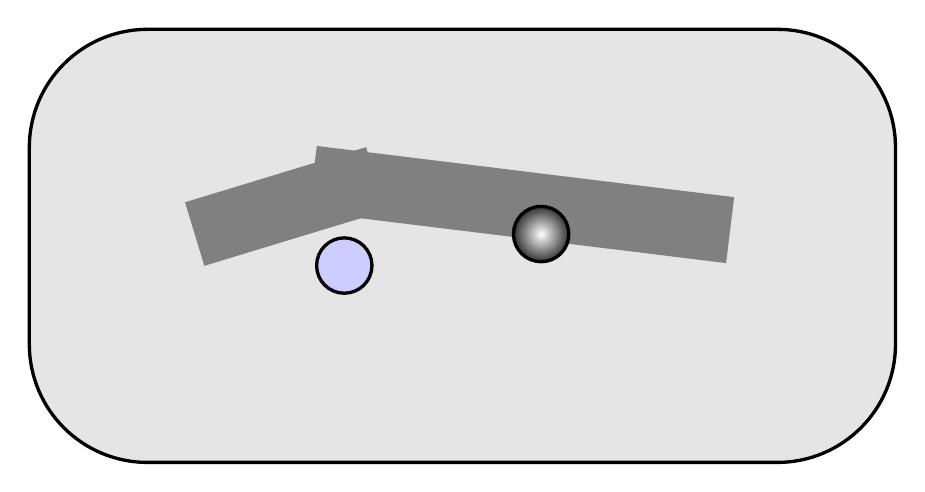
\begin{tikzpicture}
			 Background Box
			\begin{pgfonlayer}{background}
				\draw [rounded corners=1.5cm, very thick, fill=black!10] (-2.5,-3) rectangle (8.5,2.5);
			\end{pgfonlayer}
			 Folie 5
			\path[edge] (-0.4,-0.1) -- (1.9,0.6);
			\path[edge] (1.1,0.6) -- (6.4,-0.05);
			\robot at (0,0) {};
			\node[selected obstacle] at (1.5,-.5) {};
			\node[obstacle] at (4,-0.1) {};
			\goal at (6,0) {};
			\goalHelp at (1.5,.5) {};
		\end{tikzpicture}
	\end{center}
\end{frame}

\begin{frame}
	\frametitle{Router}
	\begin{center}
		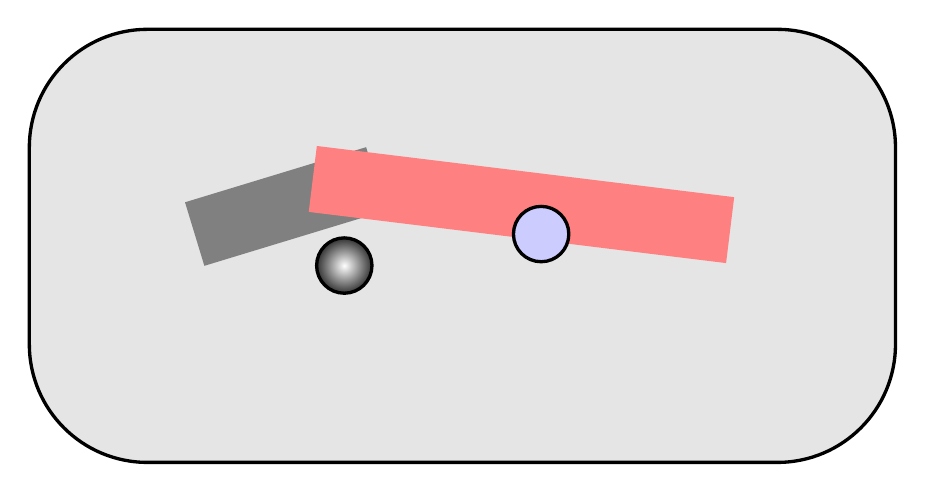
\begin{tikzpicture}
			 Background Box
			\begin{pgfonlayer}{background}
				\draw [rounded corners=1.5cm, very thick, fill=black!10] (-2.5,-3) rectangle (8.5,2.5);
			\end{pgfonlayer}
			 Folie 6
			\path[edge] (-0.4,-0.1) -- (1.9,0.6);
			\path[ignored edge] (1.1,0.6) -- (6.4,-0.05);
			\robot at (0,0) {};
			\node[obstacle] at (1.5,-.5) {};
			\node[selected obstacle] at (4,-0.1) {};
			\goal at (6,0) {};
			\goalHelp at (1.5,.5) {};
			\goalHelp at (4,.9) {};
			\goalHelp at (4,-1.1) {};
		\end{tikzpicture}
	\end{center}
\end{frame}

\begin{frame}
	\frametitle{Router}
	\begin{center}
		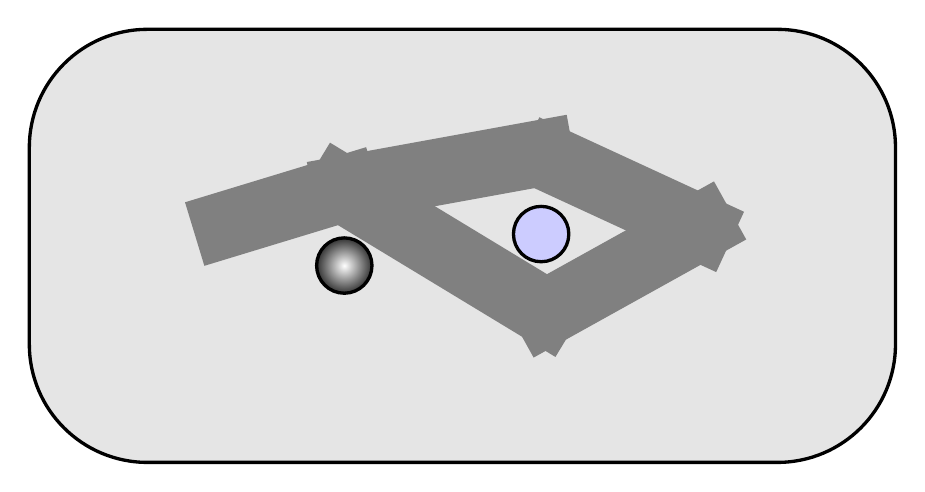
\begin{tikzpicture}
			 Background Box
			\begin{pgfonlayer}{background}
				\draw [rounded corners=1.5cm, very thick, fill=black!10] (-2.5,-3) rectangle (8.5,2.5);
			\end{pgfonlayer}
			 Folie 7
			\path[edge] (-0.4,-0.1) -- (1.9,0.6);
			\path[edge] (1.1,0.7) -- (4.4,-1.3);
			\path[edge] (1.1,0.4) -- (4.4,1);
			\path[edge] (3.7,-1.3) -- (6.4,0.2);
			\path[edge] (3.8,1) -- (6.4,-0.2);
			\robot at (0,0) {};
			\node[obstacle] at (1.5,-.5) {};
			\node[selected obstacle] at (4,-0.1) {};
			\goal at (6,0) {};
			\goalHelp at (1.5,.5) {};
			\goalHelp at (4,.9) {};
			\goalHelp at (4,-1.1) {};
		\end{tikzpicture}
	\end{center}
\end{frame}

\begin{frame}
	\frametitle{Router}
	\begin{center}
		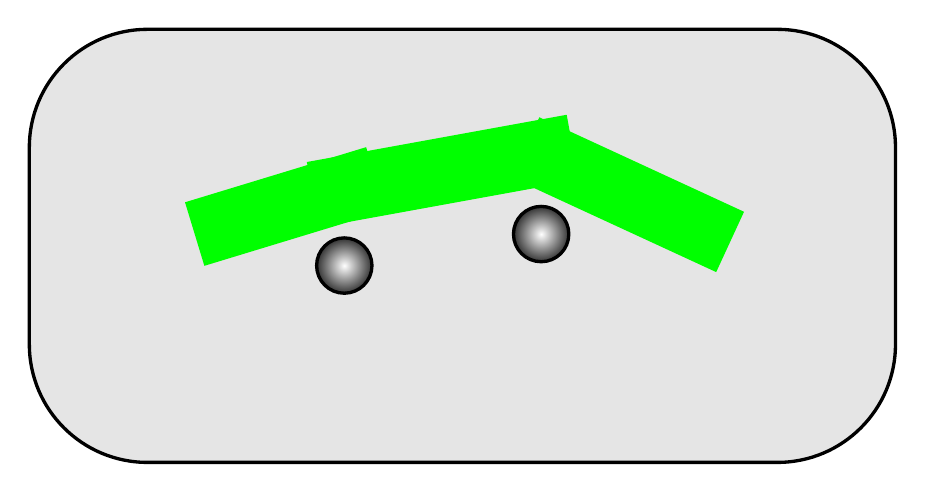
\begin{tikzpicture}
			 Background Box
			\begin{pgfonlayer}{background}
				\draw [rounded corners=1.5cm, very thick, fill=black!10] (-2.5,-3) rectangle (8.5,2.5);
			\end{pgfonlayer}
			 Folie 8
			\path[selected edge] (-0.4,-0.1) -- (1.9,0.6);
			\path[selected edge] (1.1,0.4) -- (4.4,1);
			\path[selected edge] (3.8,1) -- (6.4,-0.2);
			\robot at (0,0) {};
			\node[obstacle] at (1.5,-.5) {};
			\node[obstacle] at (4,-0.1) {};
			\goal at (6,0) {};
			\goalHelp at (1.5,.5) {};
			\goalHelp at (4,.9) {};
		\end{tikzpicture}
	\end{center}
\end{frame}

\subsection{Control}
\begin{frame}
	\frametitle{Control I}
	\textbf{Fundamental Requirements :}
	\begin{enumerate}
		\item Reach goal precisely.
		\item Drive towards goal on a straight line.
	\end{enumerate}

	\vspace{0.5cm}

	\pause

	\begin{figure}
		\centering
		\begin{overpic}[width=0.6\textwidth]{roboline.pdf}
			\put(10,39){\small Start}
			\put(10,44){\small Goal}
			\put(15,7){\small \color{blue} d}
	   	\end{overpic}
	\end{figure}
\end{frame}

\begin{frame}
	\frametitle{Control II}
	\begin{figure}
		\centering
		\begin{overpic}[width=0.8\textwidth]{control2.pdf}
			\put(30,29){\textsc{PI}}
			\put(10.5,29.75){\tiny +}
			\put(73,28){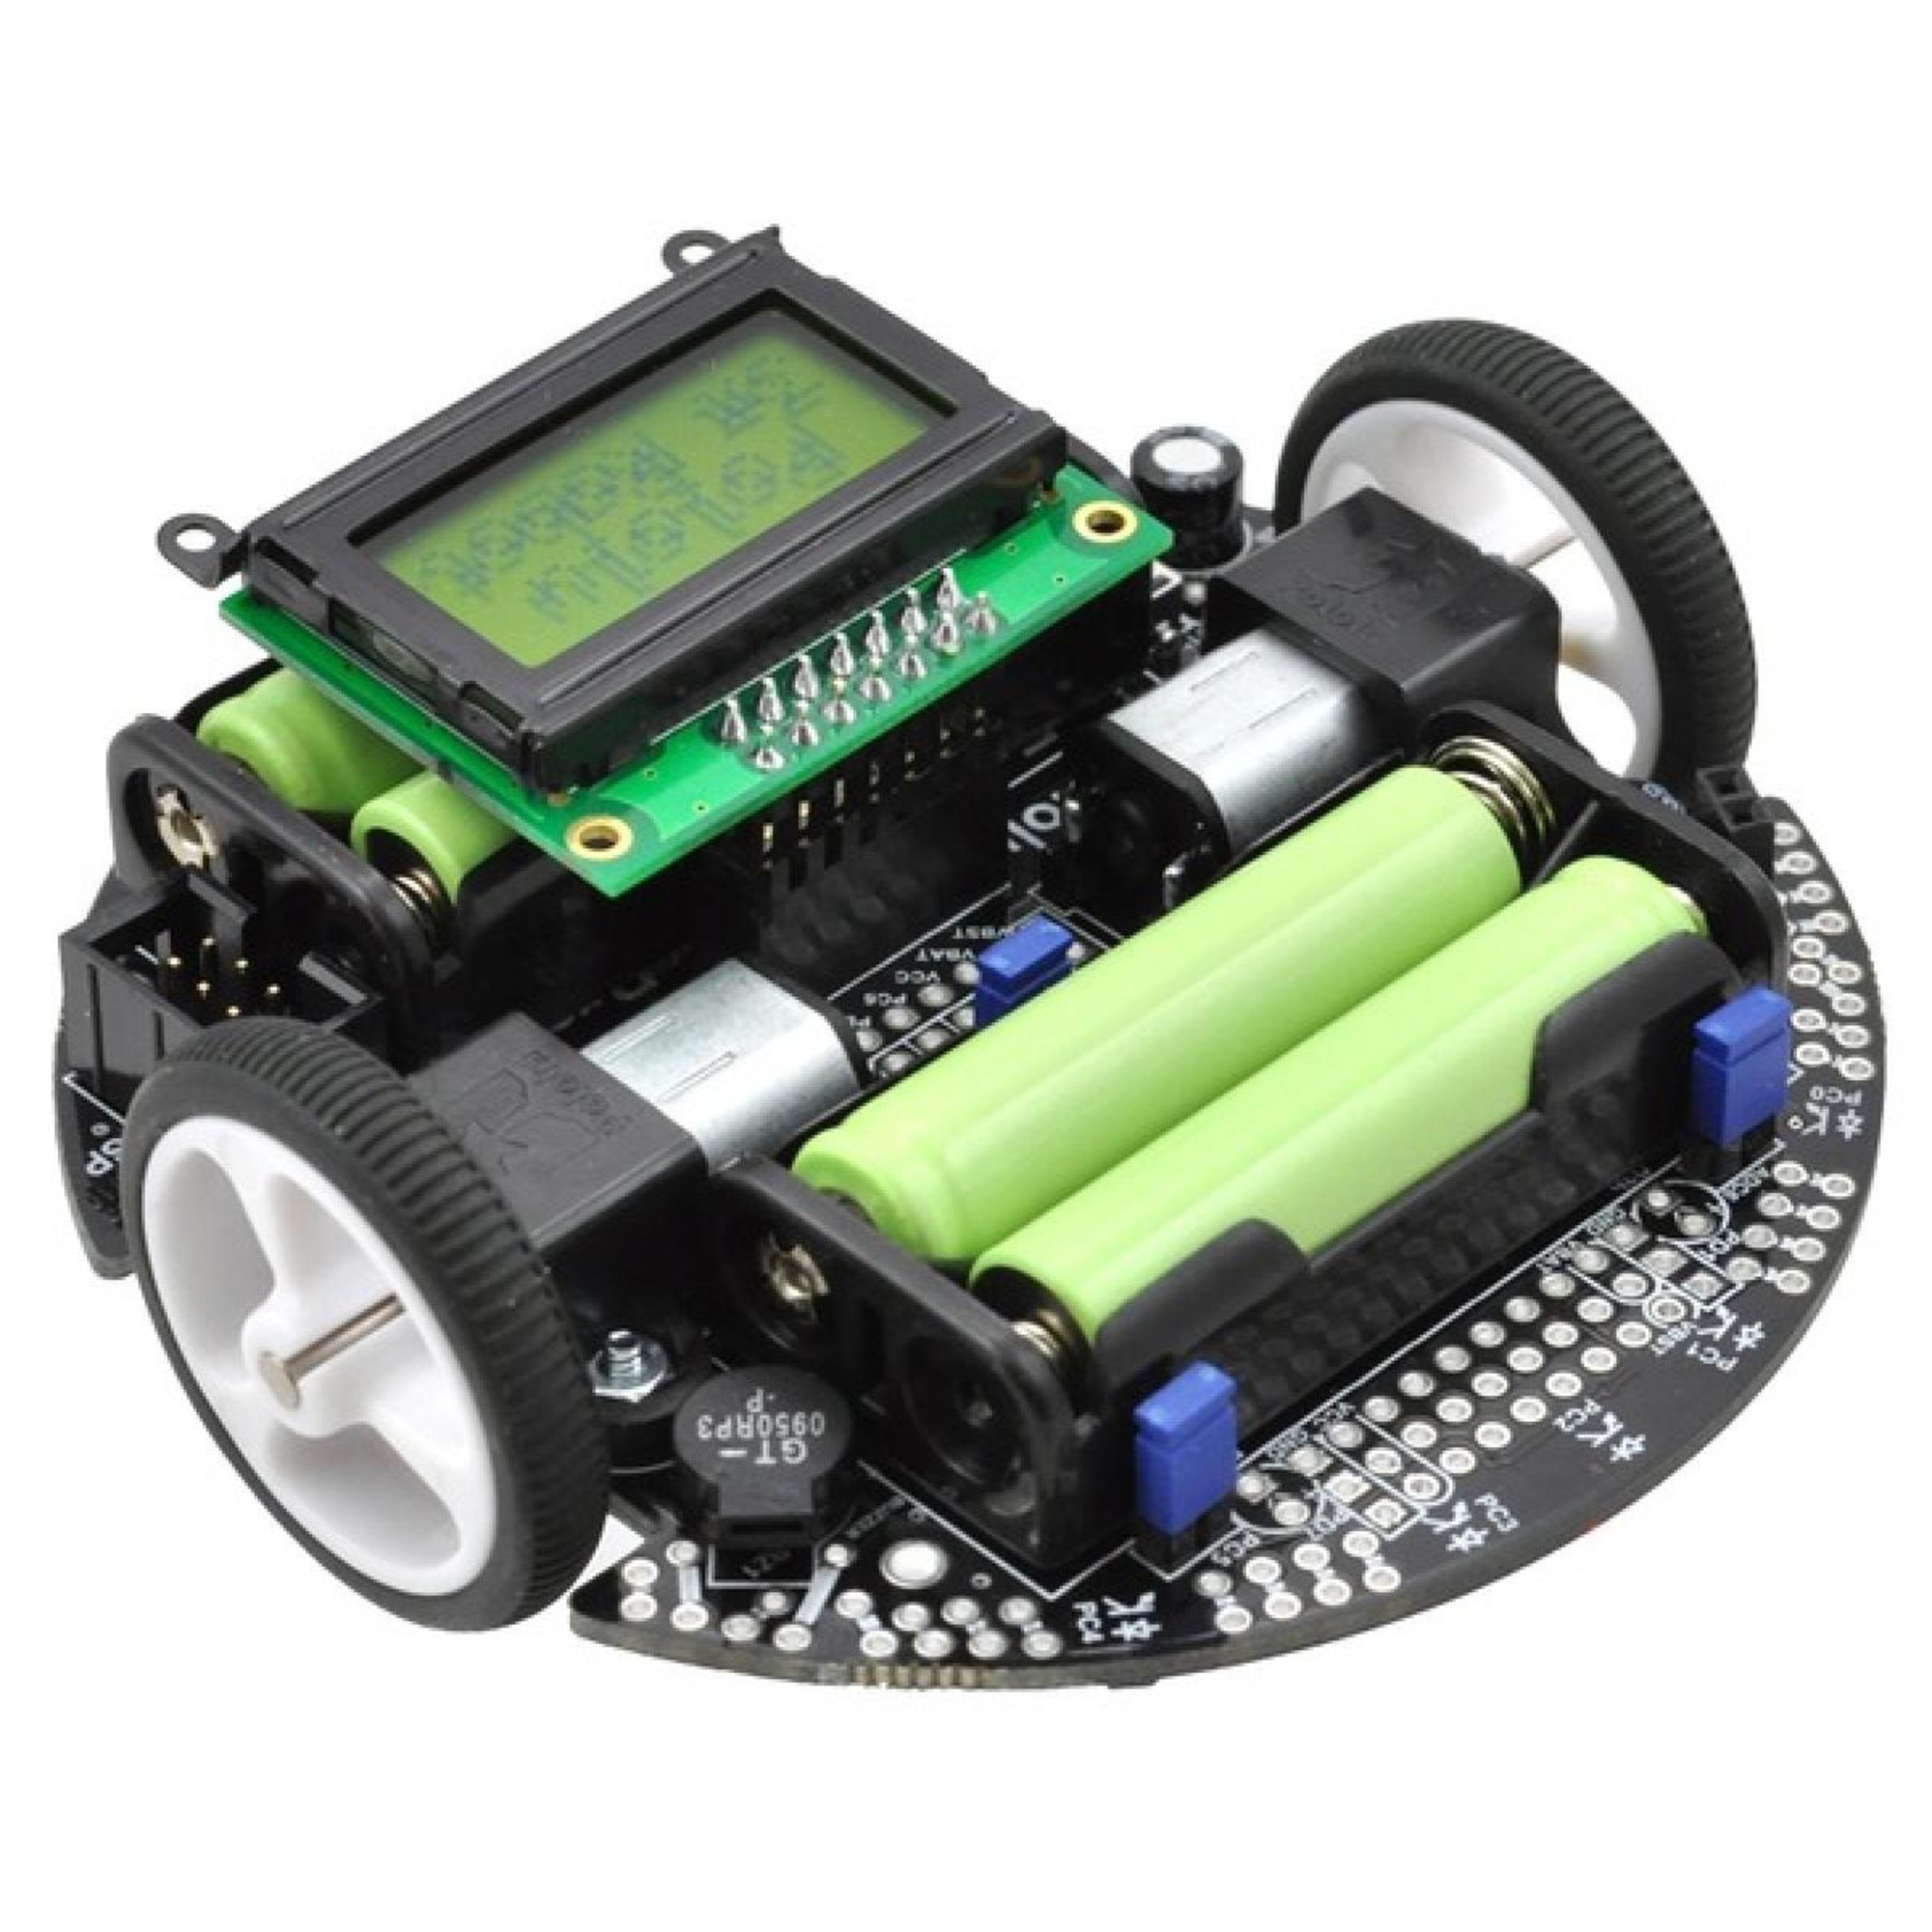
\includegraphics[scale=0.02]{3pi.pdf}}
			\put(73,25.5){\tiny Tracker}
			\put(86,32){\tiny $\left[\mathbf{x},\Omega \right]$}
			\put(60,43.5){\tiny $\Vert \mathbf{x} - \mathbf{x}_\mathrm{g} \Vert_2$}
			\put(43,29){\scriptsize $>60$}
			\put(-3,29){\small $0$}
	   	\end{overpic}
	\end{figure}
\end{frame}

\begin{frame}
	\frametitle{Control II}
	\begin{figure}
		\centering
		\begin{overpic}[width=0.8\textwidth]{control.pdf}
			\put(30,15){\textsc{PI}}
			\put(30,29){\textsc{PI}}
			\put(10.5,15.5){\tiny +}
			\put(10.5,29.75){\tiny +}
			\put(57.15,29.75){\tiny +}
			\put(73,28){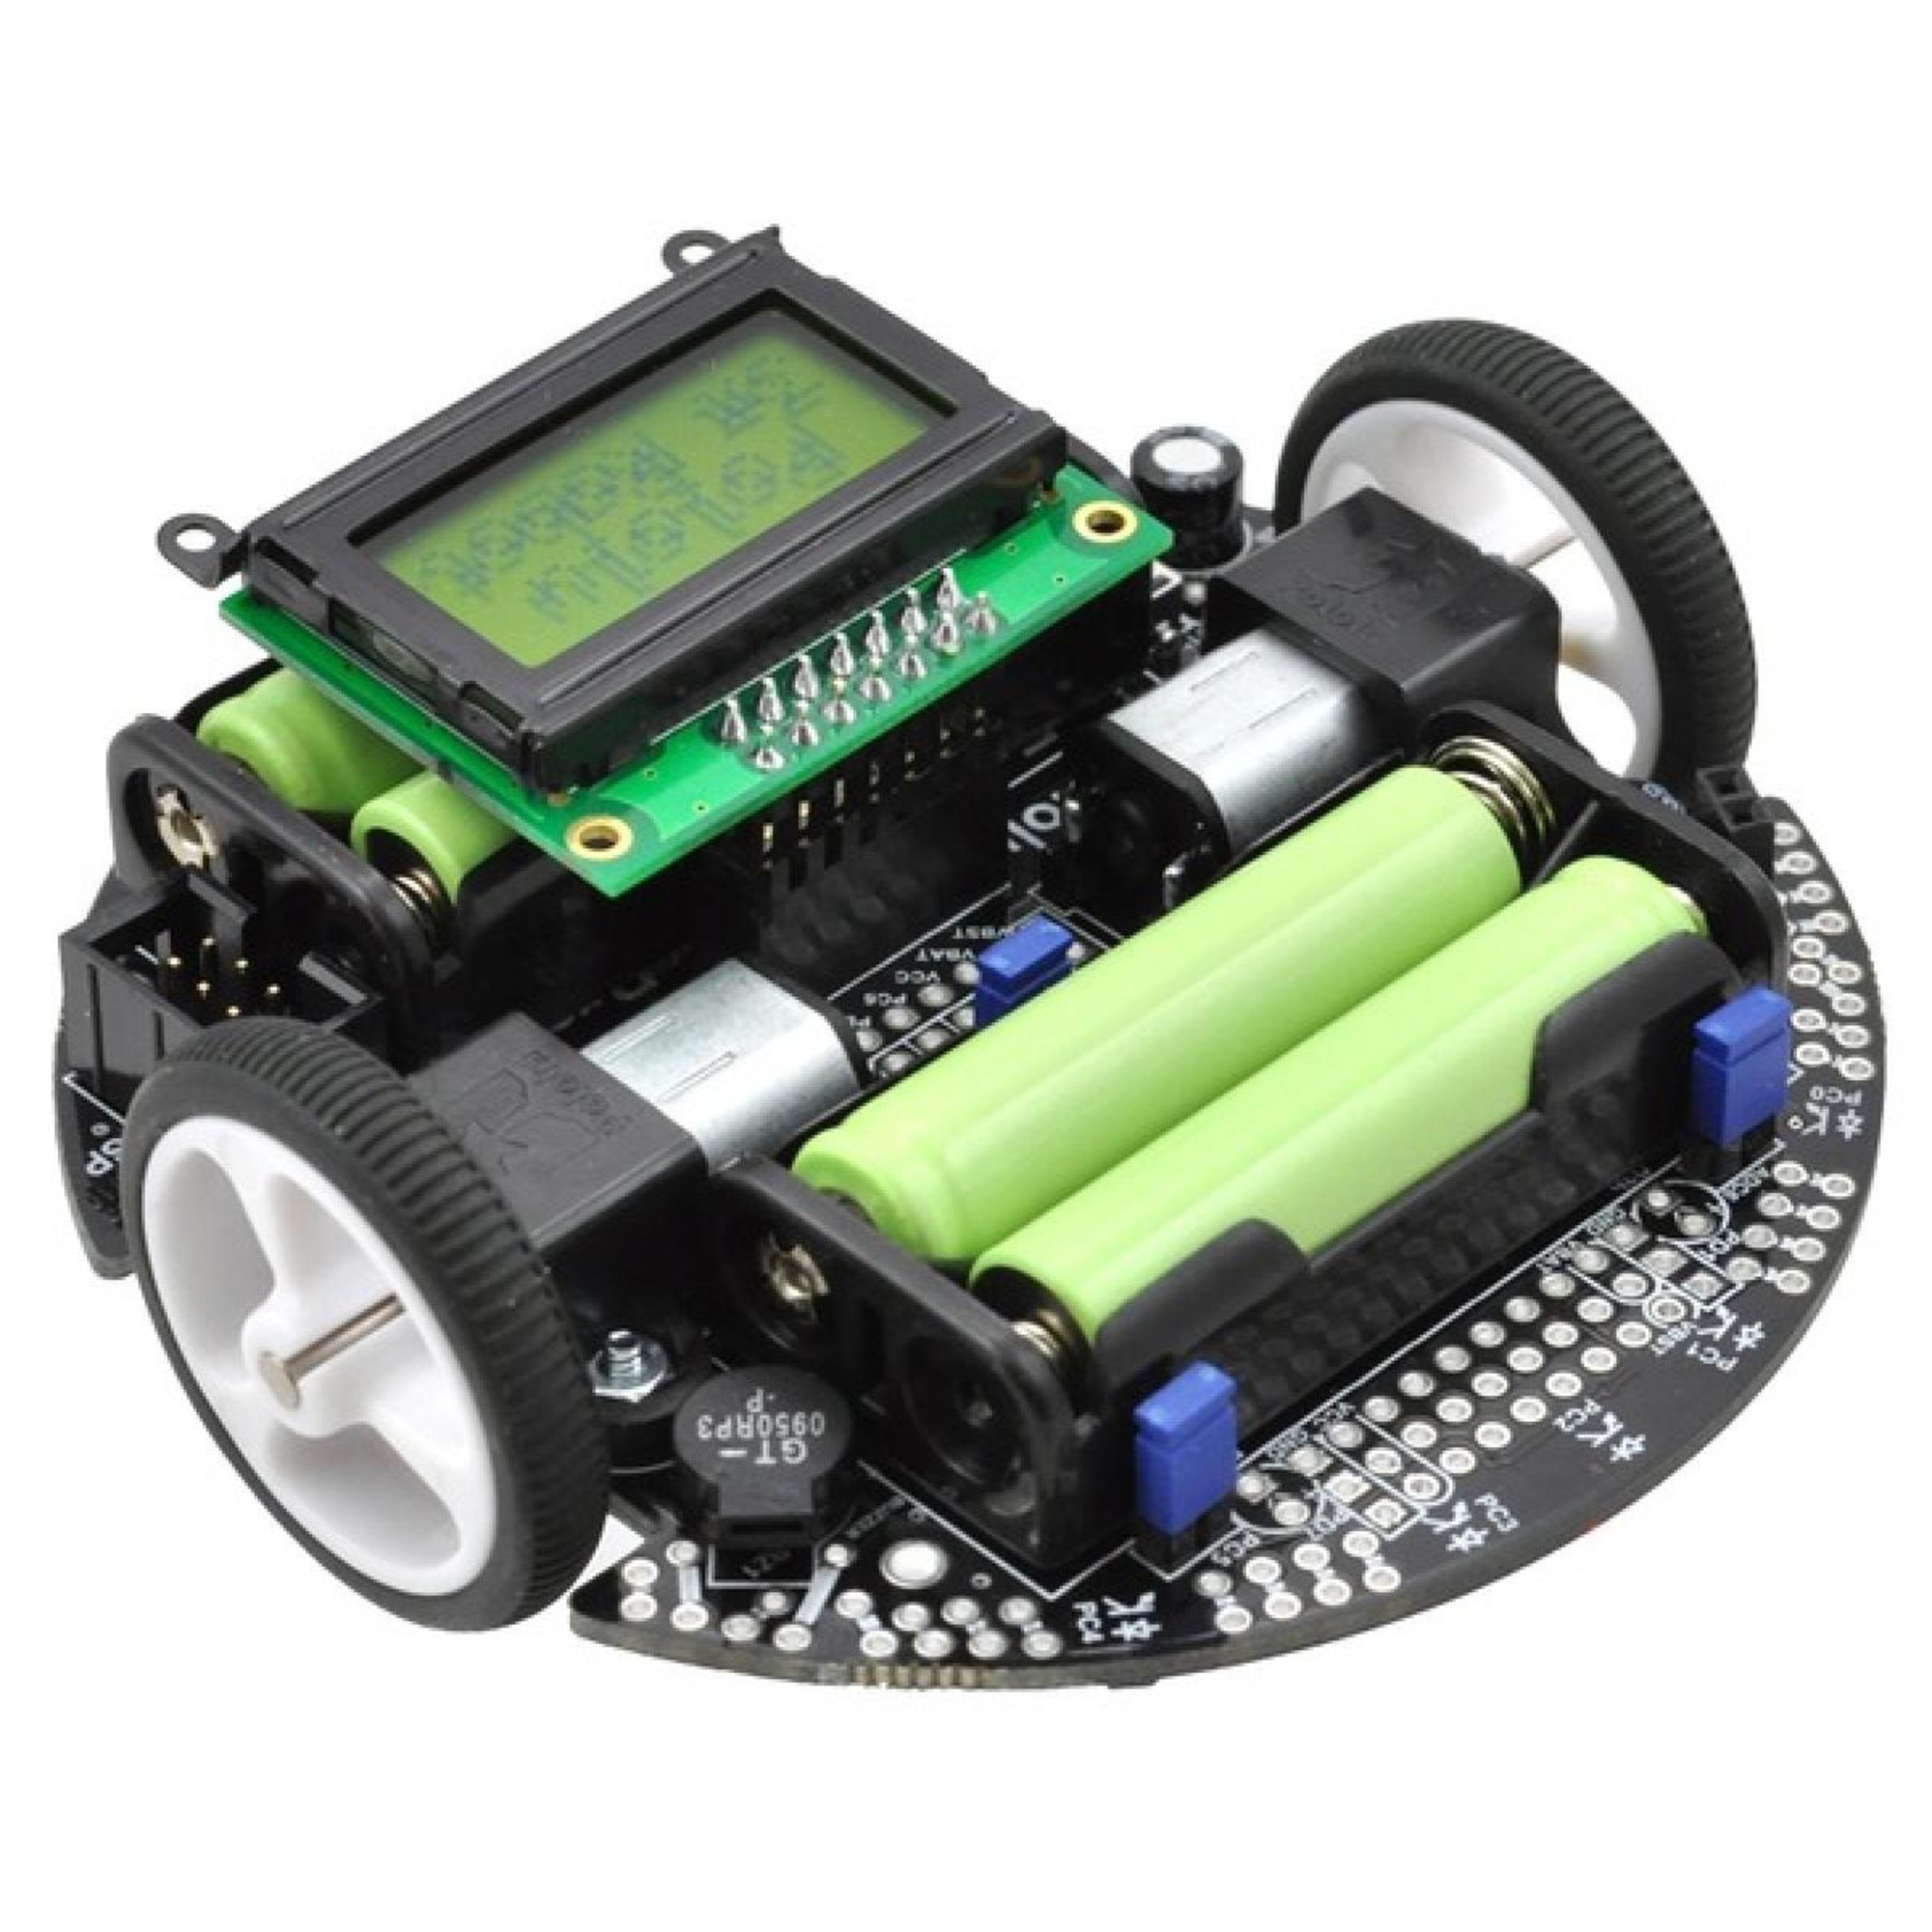
\includegraphics[scale=0.02]{3pi.pdf}}
			\put(73,25.5){\tiny Tracker}
			\put(86,32){\tiny $\left[\mathbf{x},\Omega \right]$}
			\put(60,43.5){\tiny $\Vert \mathbf{x} - \mathbf{x}_\mathrm{g} \Vert_2$}
			\put(65,1.5){\scriptsize $d$}
			\put(43,29){\scriptsize $>60$}
			\put(-3,29){\small $0$}
			\put(-3,15){\small $0$}
	   	\end{overpic}
	\end{figure}
\end{frame}

\begin{frame}
	\frametitle{Control III}
	\begin{columns}[T]
		\begin{column}{0.5\textwidth}
			\begin{center}
				\begin{tikzpicture}
					\begin{axis}[small, axis equal, grid=major, legend style={anchor=north east,font=\tiny,line width=1pt,mark size=3pt}]
			   		\addplot [blue,only marks,mark=x] table [col sep=comma] {Data/gotoC.dat};
						\addlegendentry{goto C}
						\addplot [red,only marks,mark=x] table [col sep=comma] {Data/goto_ct.dat};
						\addlegendentry{cruise to}
						\addplot [green!70!blue,only marks,mark=x] table [col sep=comma] {Data/goto_gt.dat};
						\addlegendentry{goto}
						\draw[black,very thick] (axis cs:0.375,-0.025) rectangle (axis cs:0.425,0.025);
						\draw[black,very thick] (axis cs:-0.025,0.375) rectangle (axis cs:0.025,0.425);
						\draw[black,very thick] (axis cs:-0.425,-0.025) rectangle (axis cs:-0.375,0.025);
						\draw[black,very thick] (axis cs:-0.025,-0.425) rectangle (axis cs:0.025,-0.375);
					\end{axis}
				\end{tikzpicture}
			\end{center}
		\end{column}
		\begin{column}{0.5\textwidth}
			\begin{center}
				\begin{tikzpicture}
					\begin{axis}[small, axis equal, grid=major, legend style={anchor=north east,font=\tiny,line width=1pt,mark size=3pt}]
						\addplot [red,mark=none] table [col sep=comma] {Data/goto_ct_Line.dat};
						\addplot [green!70!blue,mark=noe] table [col sep=comma] {Data/goto_gt_Line.dat};
						\addplot [blue,mark=none] table [col sep=comma] {Data/gotoC_Line.dat};
					\end{axis}
				\end{tikzpicture}
			\end{center}
		\end{column}
	\end{columns}
	\pause
	\vspace{0.3cm}
	\textbf{Average distance to desired target}\\
	\begin{center}
	goTo: 2.54 cm\hspace{1cm} CruiseTo: 5.49 cm \hspace{1cm} goto C: 0.295 cm
	\end{center}
\end{frame}

\subsection{Strategy}
\begin{frame}
    \frametitle{Overview}
    \begin{figure}
        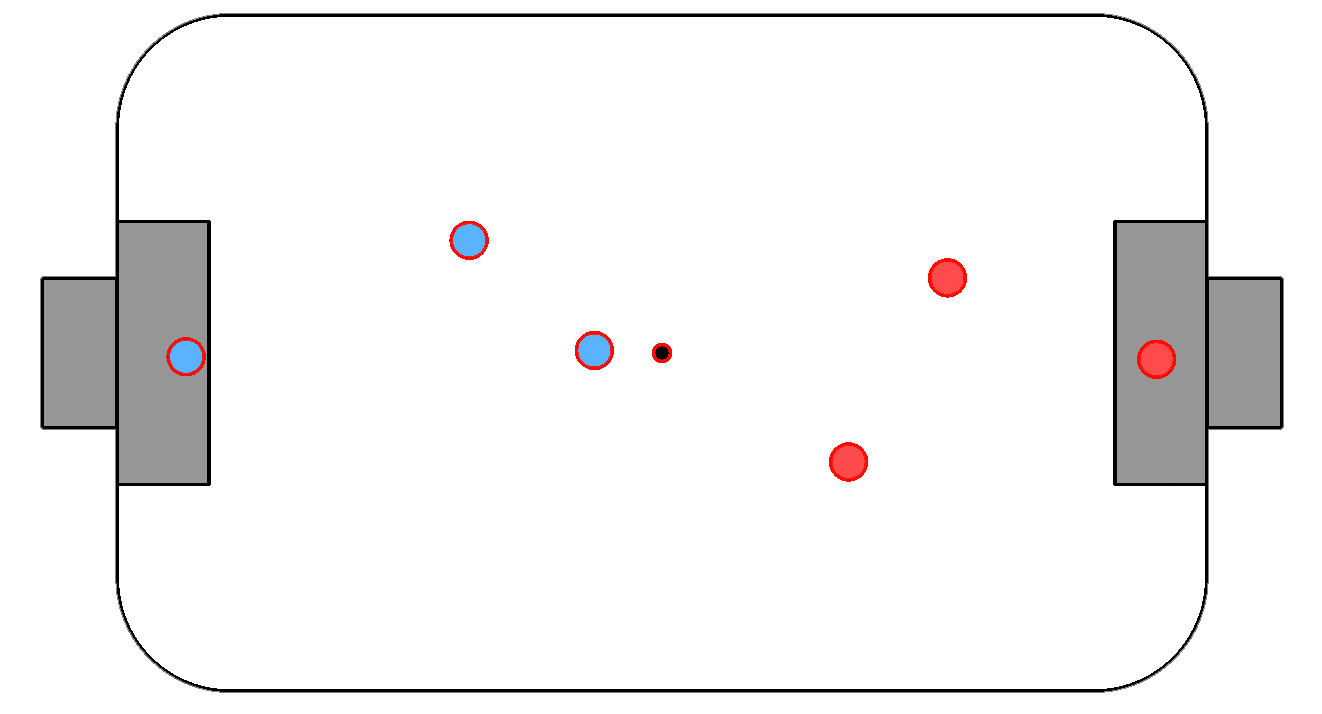
\includegraphics[width=0.7\textwidth]{Pictures/strategy}
    \end{figure}
    \textbf{Strategy:} \textit{What do we want to do?}\\
    \textbf{Tactics:} \textit{How can we achieve it?}
\end{frame}

\begin{frame}
		\frametitle{Goalkeeper Tactics I}
		\textbf{Goalkeeper:}\\
		\begin{itemize}
				\item Calculate target position depending on \textbf{ball moving direction}\\
		\end{itemize}
		\begin{center}
				%!tikz editor 1.0
%!tikz source begin
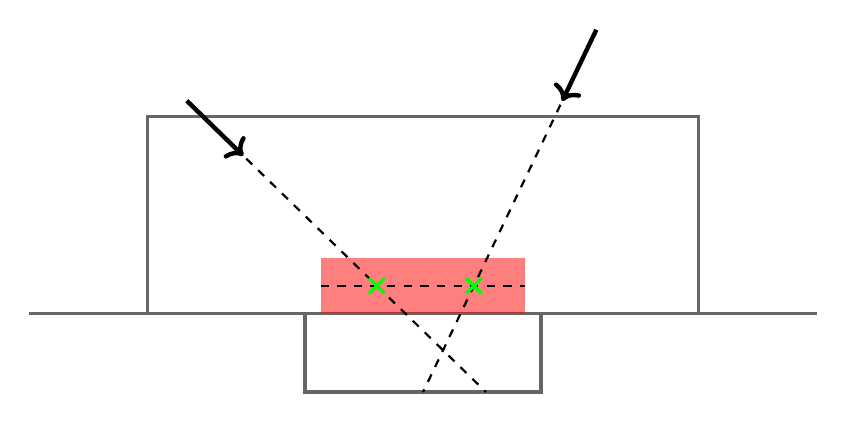
\begin{tikzpicture}
    \begin{scope}[rotate=90]
	% Background Box
	\begin{pgfonlayer}{background}
		\draw [very thick, color=black!60!white] (0,-3.5) rectangle (2.5, 3.5);
		\draw [very thick, color=black!60!white] (-1,-1.5) rectangle (0,1.5);

		\draw [very thick, color=black!60!white, rounded corners=1.5cm]  (0,-5) -- (0, 0) -- (0, 5);
%		\draw [very thick, color=black!60!white, rounded corners=1.5cm] (3,-7) -- (0,-7) -- (0, 0) -- (0, 7) -- (3,7);
	\end{pgfonlayer}

	\draw[color=red, line width=.7cm, opacity=.5] (.35, 1.3) -- (.35, -1.3);
	\draw[dashed, thick, name path=robot] (.35, 1.3) -- (.35, -1.3);

  \coordinate (ballpos1) at (3.6,-2.2);
  \coordinate (direction1) at (-1,0);
  \draw[ultra thick,->] (ballpos1) -- ($ (ballpos1)!1cm!(direction1) $);
	\draw[thick, dashed, name path=ball1] (ballpos1) -- (direction1);
	\ball at (3.6,-2.2) {};

  \coordinate (ballpos2) at (2.7,3);
  \coordinate (direction2) at (-1,-0.8);
  \draw[ultra thick,->] (ballpos2) -- ($ (ballpos2)!1cm!(direction2) $);
  \draw[thick, dashed, name path=ball2] (ballpos2) -- (direction2);
  \ball at (2.7,3) {};


	\path [name intersections={of=robot and ball1,by=x1}];
	\path [name intersections={of=robot and ball2,by=x2}];

	\draw (x1) node [cross=4pt, very thick] {};
	\draw (x2) node [cross=4pt, very thick] {};


	\robotr at (.35,1.3) {};
	\robotr at (.35,-1.3) {};
	\end{scope}
\end{tikzpicture}
%!tikz source end

		\end{center}
\end{frame}

\begin{frame}
    \frametitle{Goalkeeper Tactics II}
    \textbf{Goalkeeper:}\\
    \begin{itemize}
        \item Calculate target position depending on \textbf{ball position}\\
    \end{itemize}
    \begin{center}
        %!tikz editor 1.0
%!tikz source begin
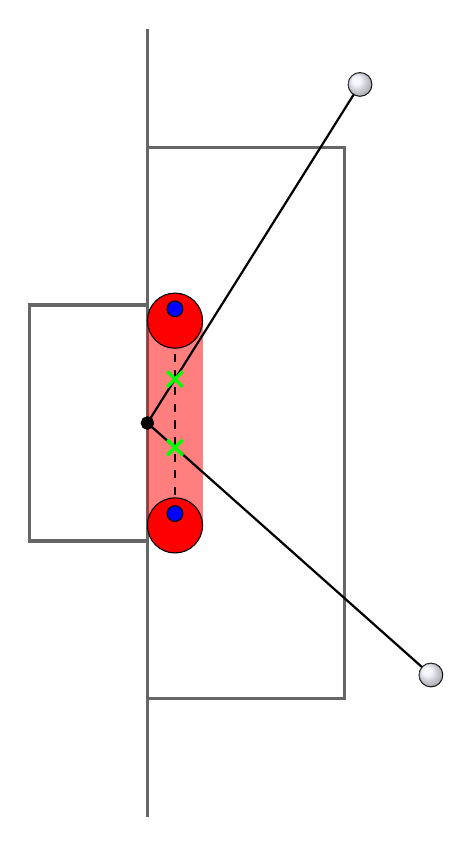
\begin{tikzpicture}
\def\robot at (#1,#2) {
	\draw[fill=red] (#1,#2) circle (0.35);
	\draw[fill=blue] (#1,#2)++(0,0.15) circle (0.1);
}
\def\ball at (#1,#2) {
	\draw [thin, fill=white] (#1,#2) circle (0.15);
	\shade[ball color=blue!10!white,opacity=0.50] (#1,#2) circle (0.15);
}

\usetikzlibrary{shapes.misc}

\tikzset{cross/.style={cross out, draw=green, minimum size=2*(#1-\pgflinewidth), inner sep=0pt, outer sep=0pt}, cross/.default={3pt}}
	

	% Background Box
	\begin{pgfonlayer}{background}
		\draw [very thick, color=black!60!white] (0,-3.5) rectangle (2.5, 3.5);
		\draw [very thick, color=black!60!white] (-1.5,-1.5) rectangle (0,1.5);
		
		\draw [very thick, color=black!60!white, rounded corners=1.5cm]  (0,-5) -- (0, 0) -- (0, 5);
%		\draw [very thick, color=black!60!white, rounded corners=1.5cm] (3,-7) -- (0,-7) -- (0, 0) -- (0, 7) -- (3,7);
	\end{pgfonlayer}
	
	\draw[color=red, line width=.7cm, opacity=.5] (.35, 1.3) -- (.35, -1.3);
	\draw[dashed, thick, name path=robot] (.35, 1.3) -- (.35, -1.3);
	
	
	\draw[thick, fill=black, name path=ball1] (3.6,-3.2) -- (0,0) circle (0.07);
	\ball at (3.6,-3.2) {};

	\draw[thick, fill=black, name path=ball2] (2.7,4.3) -- (0,0) circle (0.07);
	\ball at (2.7,4.3) {};

	
	\path [name intersections={of=robot and ball1,by=x1}];
	\path [name intersections={of=robot and ball2,by=x2}];

	\draw (x1) node [cross=4pt, very thick] {};
	\draw (x2) node [cross=4pt, very thick] {};

	
	\robot at (.35,1.3) {};
	\robot at (.35,-1.3) {};
	
\end{tikzpicture}
%!tikz source end

    \end{center}
\end{frame}

\begin{frame}
		\frametitle{Goalkeeper Tactics III}
		\textbf{Goalkeeper:}\\
		\begin{itemize}
				\item Don't move, if ball is to close to own goal\\
		\end{itemize}
		\begin{center}
				%!tikz editor 1.0
%!tikz source begin
\begin{tikzpicture}
    \begin{scope}[rotate=90]
	% Background Box
	\begin{pgfonlayer}{background}
		\draw [very thick, color=black!60!white] (0,-3.5) rectangle (2.5, 3.5);
		\draw [very thick, color=black!60!white] (-1,-1.5) rectangle (0,1.5);

		\draw [very thick, color=black!60!white, rounded corners=1.5cm]  (0,-5) -- (0, 0) -- (0, 5);
%		\draw [very thick, color=black!60!white, rounded corners=1.5cm] (3,-7) -- (0,-7) -- (0, 0) -- (0, 7) -- (3,7);
	\end{pgfonlayer}

	\ball at (0.2,0.2) {};
    
    % fake object to enlarge picture
    \draw [opacity=0.0] (3.6,-3.2) circle (0.15);

	\robotr at (.35,-1) {};
    \end{scope}
\end{tikzpicture}
%!tikz source end

		\end{center}
\end{frame}

\begin{frame}
		\frametitle{Goalkeeper Tactics IV}
		\textbf{Goalkeeper:}\\
		\begin{itemize}
				\item Angle Handlings
		\end{itemize}
		\begin{center}
				%!tikz editor 1.0
%!tikz source begin
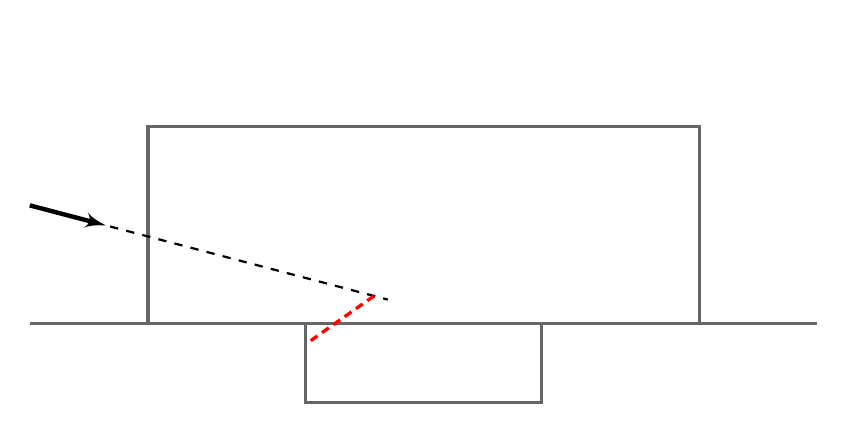
\begin{tikzpicture}
    \begin{scope}[rotate=90]
	% Background Box
	\begin{pgfonlayer}{background}
		\draw [very thick, color=black!60!white] (0,-3.5) rectangle (2.5, 3.5);
		\draw [very thick, color=black!60!white] (-1,-1.5) rectangle (0,1.5);

		\draw [very thick, color=black!60!white, rounded corners=1.5cm]  (0,-5) -- (0, 0) -- (0, 5);
%		\draw [very thick, color=black!60!white, rounded corners=1.5cm] (3,-7) -- (0,-7) -- (0, 0) -- (0, 7) -- (3,7);
	\end{pgfonlayer}

%	\draw[color=red, line width=.7cm, opacity=.5] (.35, 1.3) -- (.35, -1.3);
	\draw[dashed, thick, name path=robot, opacity=0] (.35, 1.3) -- (.35, -1.3);

	\draw[opacity=0] (3.6,-2.2) circle (0.15);

	\coordinate (ballpos2) at (1.5,5);
	\coordinate (direction2) at (-0.5,-2.6);
	\draw[ultra thick,->, >=latex'] (ballpos2) -- ($ (ballpos2)!1cm!(direction2) $);
	\draw[thick, dashed, name path=ball2] (ballpos2) -- ($ (ballpos2)!4.7cm!(direction2) $);
	\ball at (1.5,5) {};

	\path [name intersections={of=robot and ball2,by=x2}];
	\draw [very thick, densely dashed, red] (x2) -- ($(x2)!1cm!-130:(direction2)$);

%	\draw (x2) node [cross=4pt, very thick] {};

	\robotr at (.35,0.3) {};
	\end{scope}
\end{tikzpicture}
%!tikz source end

		\end{center}
\end{frame}

\begin{frame}
		\frametitle{Goalkeeper Tactics IV}
		\textbf{Goalkeeper:}\\
		\begin{itemize}
				\item Angle Handlings
		\end{itemize}
		\begin{center}
				%!tikz editor 1.0
%!tikz source begin
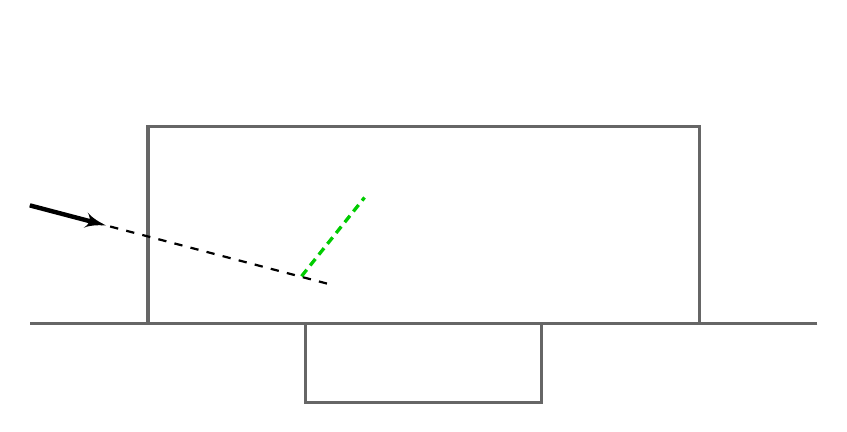
\begin{tikzpicture}
    \begin{scope}[rotate=90]
	% Background Box
	\begin{pgfonlayer}{background}
		\draw [very thick, color=black!60!white] (0,-3.5) rectangle (2.5, 3.5);
		\draw [very thick, color=black!60!white] (-1,-1.5) rectangle (0,1.5);

		\draw [very thick, color=black!60!white, rounded corners=1.5cm]  (0,-5) -- (0, 0) -- (0, 5);
%		\draw [very thick, color=black!60!white, rounded corners=1.5cm] (3,-7) -- (0,-7) -- (0, 0) -- (0, 7) -- (3,7);
	\end{pgfonlayer}

%	\draw[color=red, line width=.7cm, opacity=.5] (.35, 1.3) -- (.35, -1.3);
	\draw[dashed, thick, name path=robot, opacity=0] (.35, 1.3) -- (.35, -1.3);

	\draw[opacity=0] (3.6,-2.2) circle (0.15);

	\coordinate (ballpos2) at (1.5,5);
	\coordinate (direction2) at (-0.5,-2.6);
	\draw[ultra thick,->, >=latex'] (ballpos2) -- ($ (ballpos2)!1cm!(direction2) $);
	\draw[thick, dashed, name path=ball2] (ballpos2) -- ($ (ballpos2)!4cm!(direction2) $);
	\ball at (1.5,5) {};

	\draw [very thick, densely dashed, green!80!black] (.6,1.55) -- +(1,-.8);

%	\draw (x2) node [cross=4pt, very thick] {};

	\robotr at (.35,1.3) {};
	\end{scope} 	
\end{tikzpicture}
%!tikz source end

		\end{center}
\end{frame}

\begin{frame}
    \frametitle{Solution}
    \textbf{Goalkeeper:}\\
    \begin{itemize}
        \item Calculate target position depending on\\
        \begin{itemize}
            \item ball moving direction\\
            \item ball position\\
        \end{itemize}
        \item Don't move, if ball is to close to own goal\\
        \item Fixed robot
    \end{itemize}
    \textbf{Field players:}\\
    \begin{itemize}
        \item \textbf{One} strategy for both field players
        \item \textbf{Small} binary decision tree
        \item Recalculated each iteration
        \item Depending on ball and robot positions
    \end{itemize}
\end{frame}

\begin{frame}
    \frametitle{Decision Tree}
    \begin{center}
        %!tikz editor 1.0
%!tikz source begin
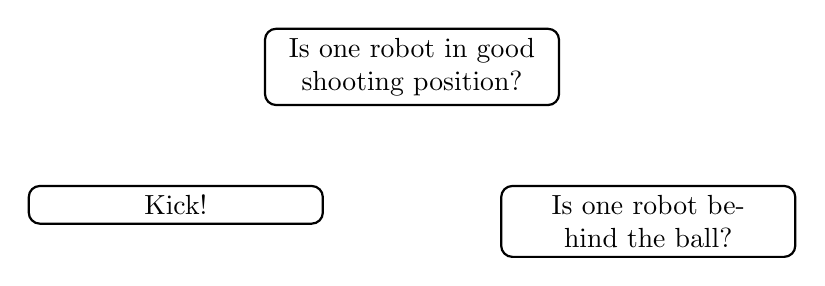
\begin{tikzpicture}
	\font\btt=rm-lmtk10
	\definecolor{PresiBlue}{RGB}{50,57,171}
	
	\tikzstyle{class}=[
		rectangle, draw=black, rounded corners, 
		text centered, anchor=north, text=black, text width=3.5cm, thick]

	\node (isgoodkickposition) [class] {Is one robot in good shooting position?};
	\node (kick) [class, below = of isgoodkickposition, xshift=-3.0cm]{Kick!};

	\node (isbehindball) [class, below = of isgoodkickposition, xshift=3.0cm]{Is one robot behind the ball?};
	
\end{tikzpicture}
%!tikz source end

    \end{center}
\end{frame}

\begin{frame}
    \frametitle{Tactics}
    \textbf{Get behind Ball}
    	\begin{center}
		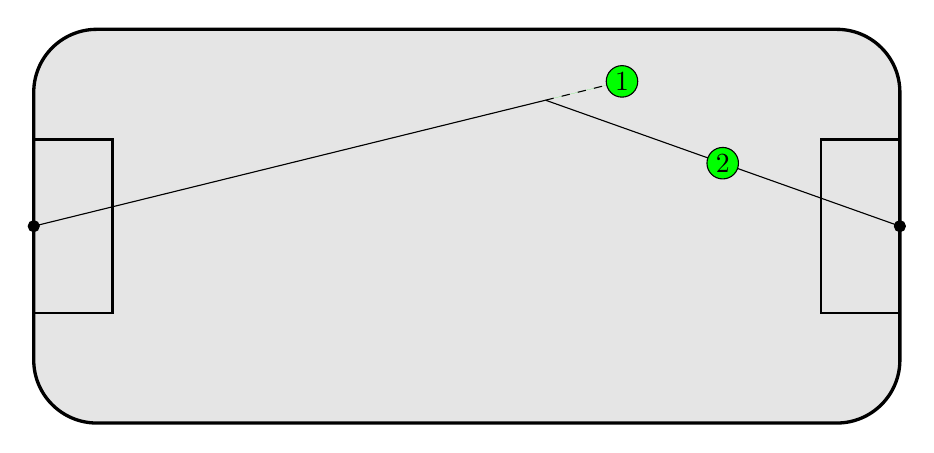
\begin{tikzpicture}
			% Background Box
			\begin{pgfonlayer}{background}
				\draw [rounded corners=.8cm, very thick, fill=black!10] (-5.5,-2.5) rectangle (5.5,2.5);
				\draw [thick] (-5.5, -1.1) rectangle (-4.5, 1.1);
				\draw [thick] (5.5, -1.1) rectangle (4.5, 1.1) (0,-2.5);
			\end{pgfonlayer}

			\coordinate (ball) at (1,1.6);
			\coordinate (enemygoal) at (-5.5,0);
			\coordinate (owngoal) at (5.5,0);

			\draw[fill=black] (ball) -- (enemygoal) circle (0.07);
			\draw[fill=green, dashed] (ball) -- ($(ball)!-1cm!(enemygoal)$);
			\draw[fill=green] ($(ball)!-1cm!(enemygoal)$) circle (0.2) node {1};

			\draw[fill=black] (ball) -- (owngoal) circle (0.07);
			\draw[fill=green] ($(ball)!.5!(owngoal)$) circle (0.2) node {2};

			\ball at (1,1.6) {};

		\end{tikzpicture}
	\end{center}
\end{frame}

\begin{frame}
    \frametitle{Tactics}
    \textbf{Follow Ball}
    	\begin{center}
		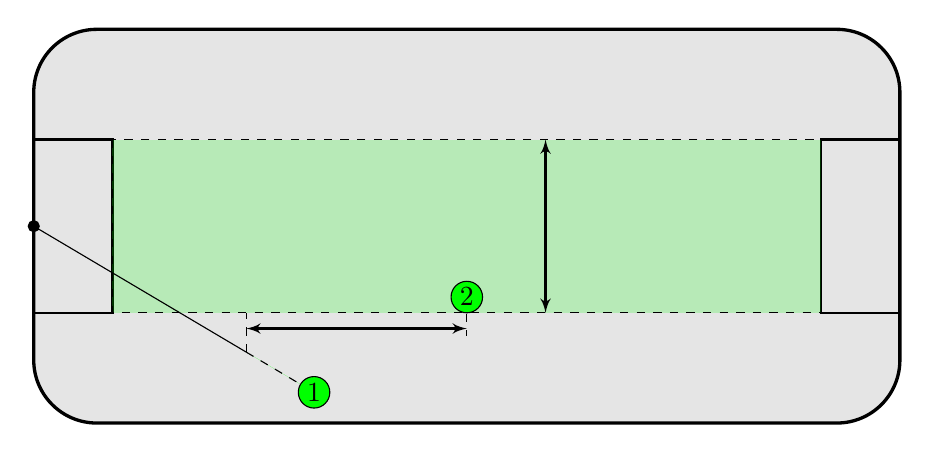
\begin{tikzpicture}
			% Background Box
			\begin{pgfonlayer}{background}
				\draw [rounded corners=.8cm, very thick, fill=black!10] (-5.5,-2.5) rectangle (5.5,2.5);
				\draw [thick] (-5.5, -1.1) rectangle (-4.5, 1.1);
				\draw [thick] (5.5, -1.1) rectangle (4.5, 1.1);
			\end{pgfonlayer}

			\coordinate (ball) at (-2.8,-1.6);
			\coordinate (enemygoal) at (-5.5,0);
			\coordinate (owngoal) at (5.5,0);

			\draw [dashed, fill=green, fill opacity=0.2] (-4.5, 1.1) rectangle (4.5, -1.1);
			\draw [<->, >=latex', thick] (1,1.1) -- (1,-1.1);

			\draw[fill=black] (ball) -- (enemygoal) circle (0.07);
			\draw[fill=green, dashed] (ball) -- ($(ball)!-1cm!(enemygoal)$);
			\draw[fill=green] ($(ball)!-1cm!(enemygoal)$) circle (0.2) node {1};

			\draw [dashed] (ball) -- ++(0,0.5) (0,-0.9) -- ++(0,-0.5);
			\draw [<->, >=latex', thick] (0,-1.1) ++(0,-0.2) -- ++(-2.8,0);

			\draw[fill=green] (0,-0.9) circle (0.2) node {2};

			\ball at (-2.8,-1.6) {};

		\end{tikzpicture}
	\end{center}
\end{frame}

%\begin{frame}
%    \frametitle{Class Diagramm}
%    \begin{center}
%        %!tikz editor 1.0
%!tikz source begin
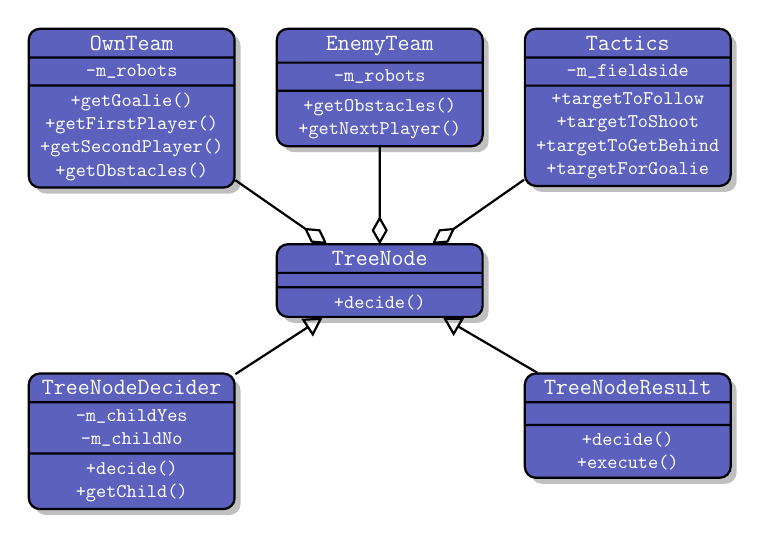
\begin{tikzpicture}[node distance=4.5cm, scale=0.7, transform shape]
	\font\btt=rm-lmtk10
	\definecolor{PresiBlue}{RGB}{50,57,171}
	
	\tikzstyle{class}=[
		rectangle, draw=black, rounded corners, rectangle split, rectangle split parts=3, 
		fill=PresiBlue!80, drop shadow, font=\tt,
        text centered, anchor=north, text=white, text width=3.5cm, thick]
		
	\tikzstyle{inheritance}=[draw, ->, >=open triangle 60, thick]
	\tikzstyle{property}=[draw, ->, >=open diamond, thick]
	\tikzstyle{line}=[-, thick]
   
   % Classes
      
	\node (treenode) [class]
	{
		{\large \texttt{\textbf{TreeNode}}}
		
		\nodepart{second}
		
		\nodepart{third}
		+decide()
	};
	
	\node (treenodedecider) [class, left =of treenode.south, anchor = north, yshift=-1cm]
	{
		{\large \texttt{\textbf{TreeNodeDecider}}}
		
		\nodepart{second}
		-m\char`_childYes\\
		-m\char`_childNo
		
		\nodepart{third}
		+decide()\\
		+getChild()
	} edge [inheritance] (treenode);
	
	\node (treenoderesult) [class, right =of treenode.south, anchor = north, yshift=-1cm]
	{
		{\large \texttt{\textbf{TreeNodeResult}}}
		\nodepart{third}
		+decide()\\
		+execute()		
	} edge [inheritance] (treenode);

	\node (ownteam) [class, left = of treenode.north, anchor = south, yshift=1cm]
	{
		{\large \texttt{\textbf{OwnTeam}}}
		
		\nodepart{second}
		-m\char`_robots
		
		\nodepart{third}
		+getGoalie()\\
		+getFirstPlayer()\\
		+getSecondPlayer()\\
		+getObstacles()
		
	} edge [property] (treenode);

	\node (enemyteam) [class, right = of ownteam.north, anchor = north]
	{
		{\large \texttt{\textbf{EnemyTeam}}}

		\nodepart{second}
		-m\char`_robots
		
		\nodepart{third}
		+getObstacles()\\
		+getNextPlayer()

	} edge [property] (treenode);

	\node (tactics) [class, right = of enemyteam.north, anchor = north]
	{
		{\large \texttt{\textbf{Tactics}}}
		
		\nodepart{second}
		-m\char`_fieldside
		
		\nodepart{third}
		+targetToFollow\\
		+targetToShoot\\
		+targetToGetBehind\\
		+targetForGoalie
	} edge [property] (treenode);


	% Connections
	
	
\end{tikzpicture}
%!tikz source end

%    \end{center}
%\end{frame}

\subsection{GUI Tool}
\begin{frame}
    \frametitle{Validation GUI}
    \begin{figure}
        \center
        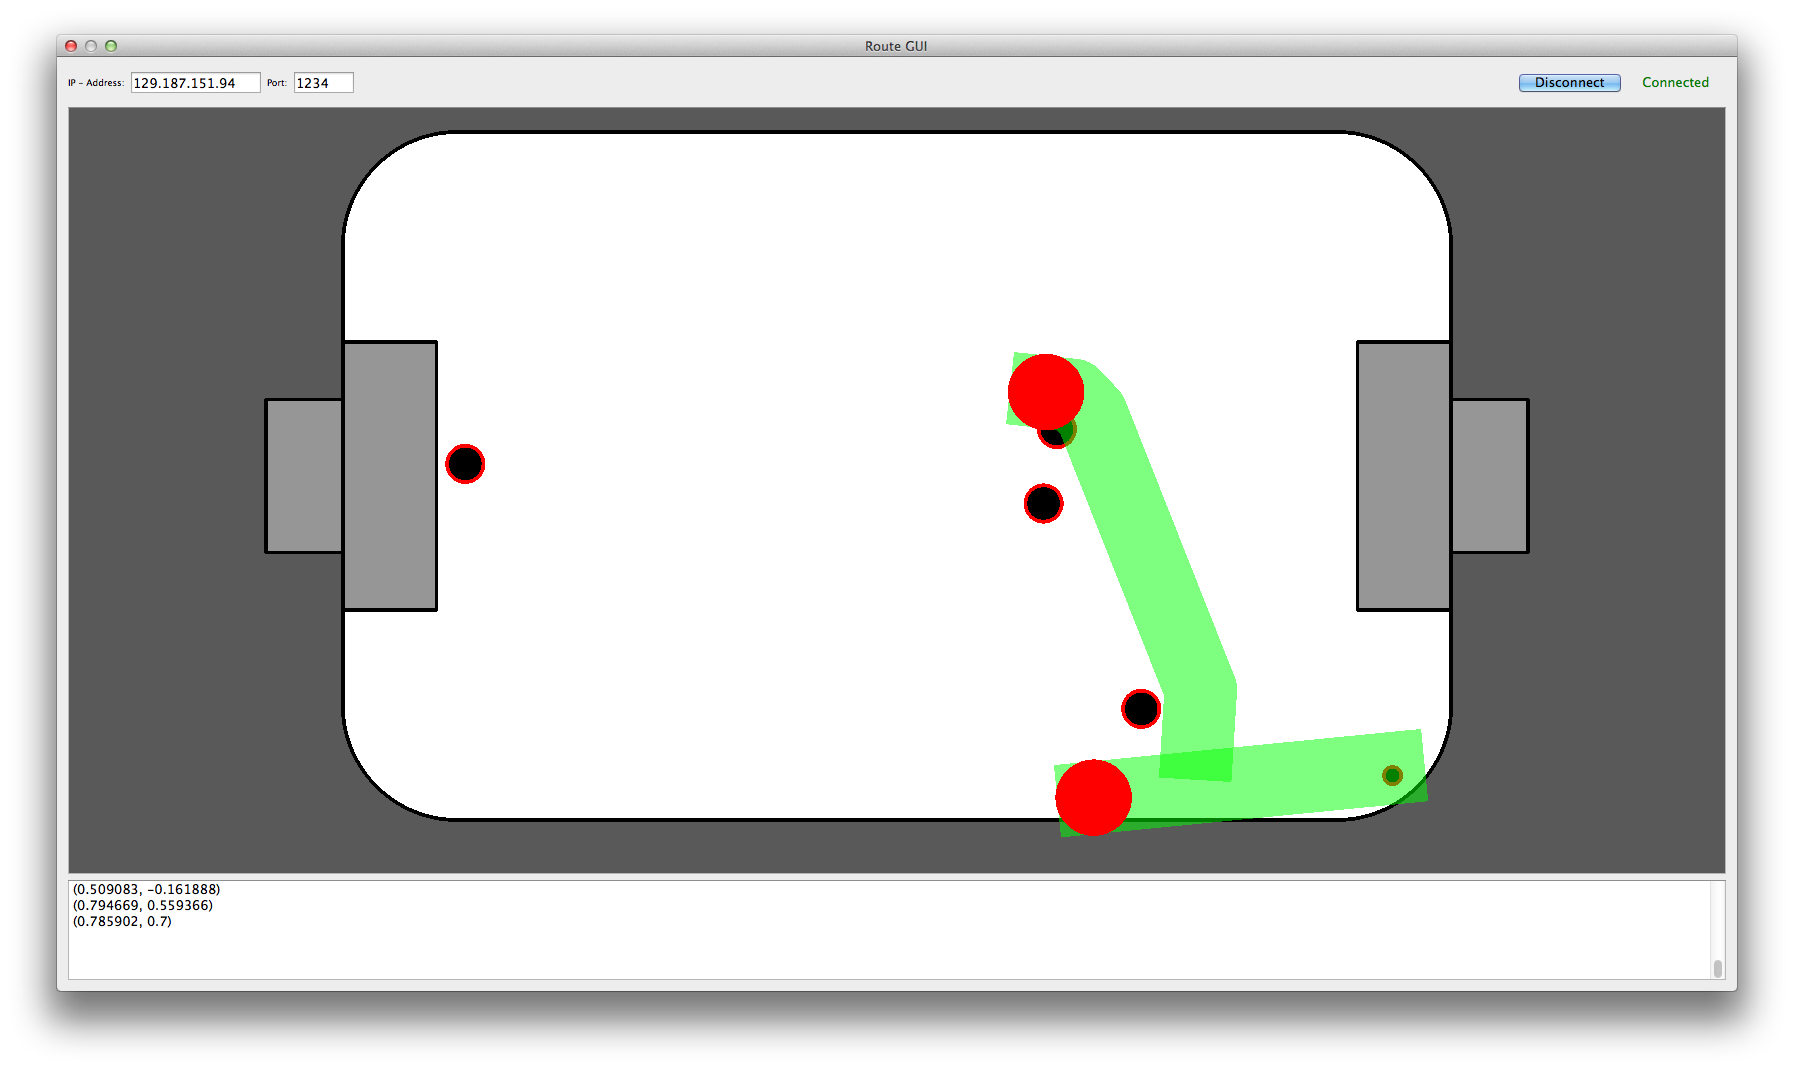
\includegraphics[width=0.95\textwidth]{Pictures/gui-big}
    \end{figure}

\end{frame}

\begin{frame}
    \frametitle{Validation GUI}
    \begin{columns}[T]
        \begin{column}{0.4\textwidth}
            \begin{figure}
                \center
                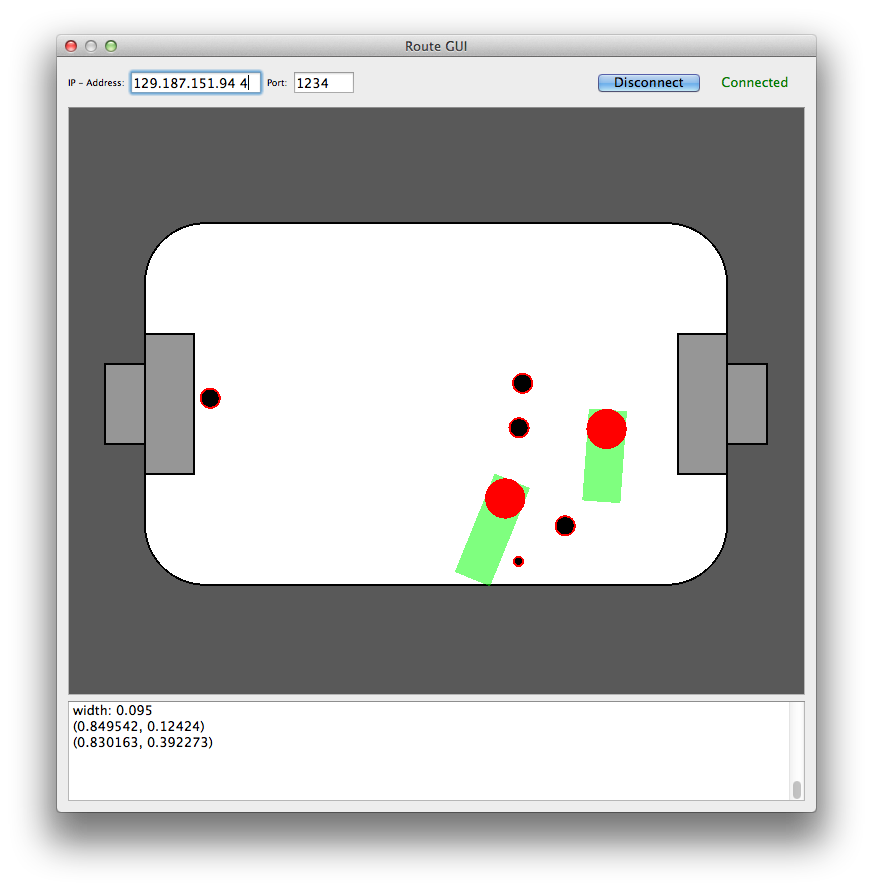
\includegraphics[width=\textwidth]{Pictures/gui-small}
            \end{figure}
        \end{column}
        \begin{column}{0.6\textwidth}
            \textbf{Features:}
            \begin{itemize}
                \item Connects via \textbf{network}
                \item Updates \textbf{live and in realtime}
                \item Shows own robots and \textbf{routes}
                \item Displays all obstacles
                \item Logs positions
            \end{itemize}
        \end{column}
    \end{columns}
\end{frame}

\begin{frame}
    \frametitle{Validation GUI}
    \begin{columns}[T]
        \begin{column}{0.4\textwidth}
            \begin{figure}
                \center
                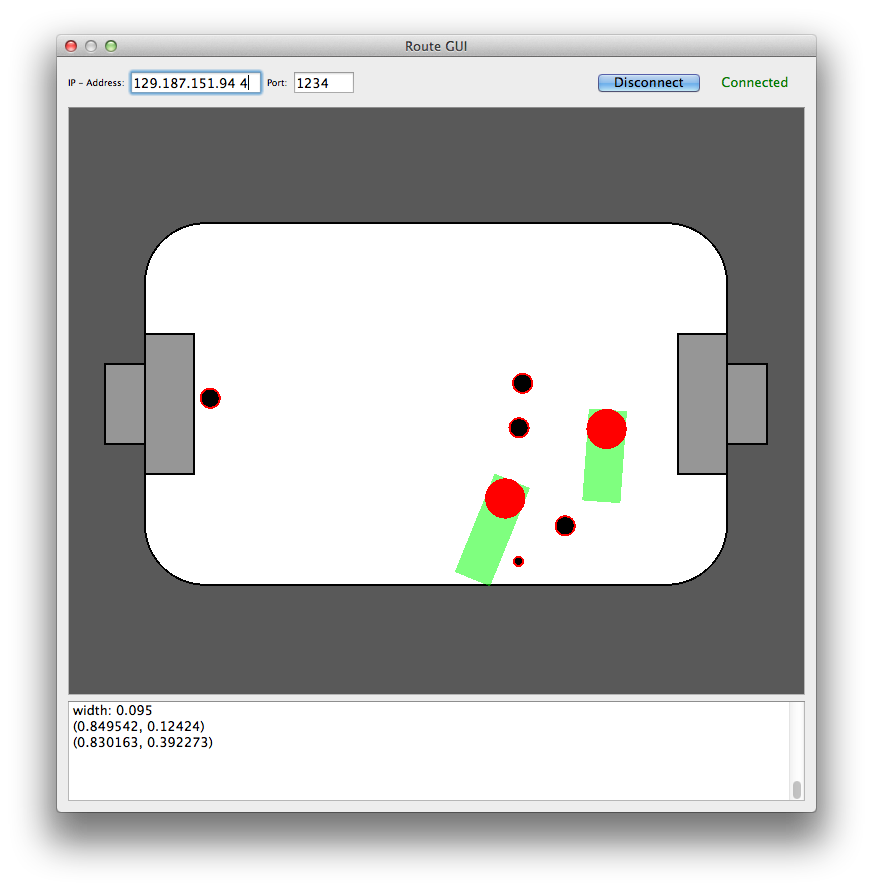
\includegraphics[width=\textwidth]{Pictures/gui-small}
            \end{figure}
        \end{column}
        \begin{column}{0.6\textwidth}
            \textbf{Implementation:}
            \begin{itemize}
                \item Seperate \textsc{Qt 5} project
                \item Connection via TCP/IP Socket
                \item Drawing on \textsc{QGraphicsView}
            \end{itemize}
        \end{column}
    \end{columns}
\end{frame}

\begin{frame}
    \frametitle{Demo: Video}
	\centering
	\movie[showcontrols]{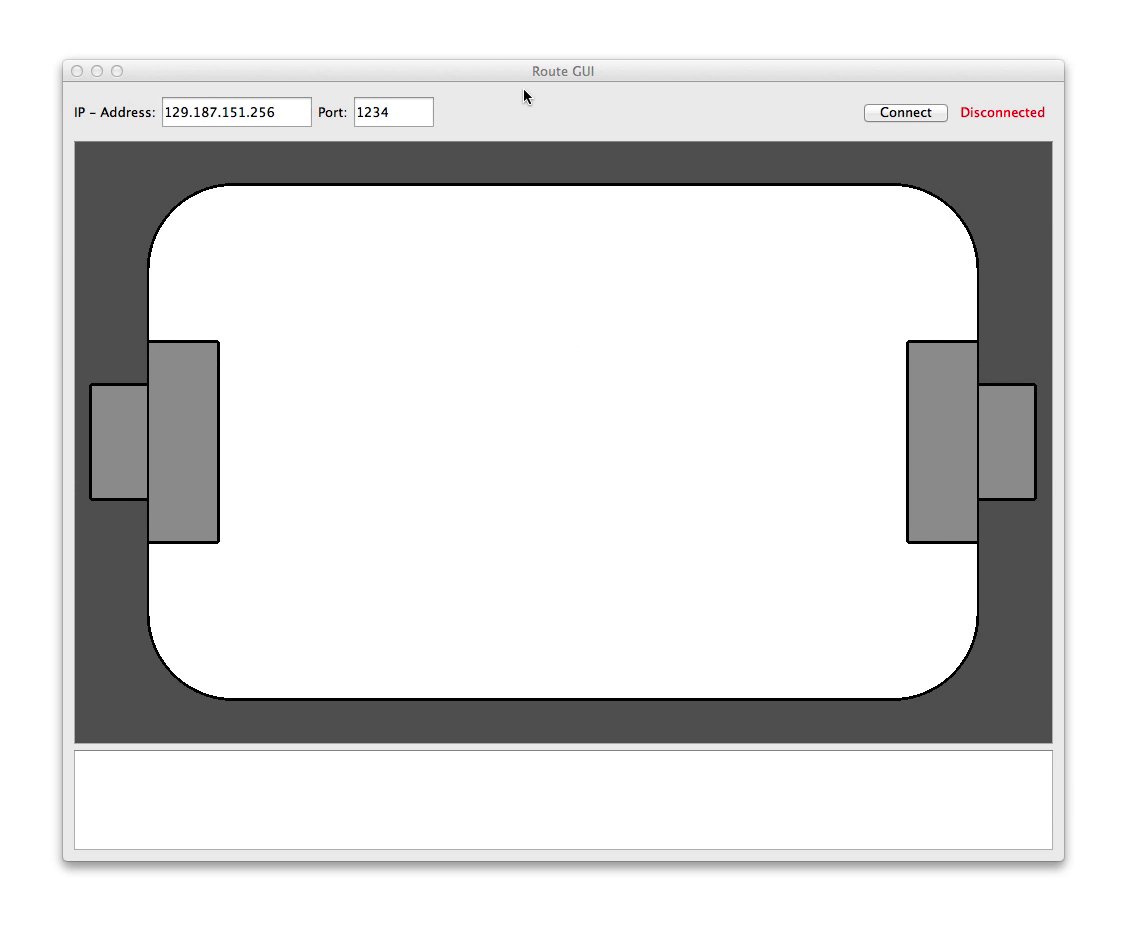
\includegraphics[height=0.8\textheight]{Pictures/gui_demo_preview.png}}{Pictures/gui_demo.mov}
\end{frame}

\section{Results}
\subsection{Time Schedule}
\begin{frame}
	\frametitle{Gantt Chart I}
	\begin{figure}
		\centering
		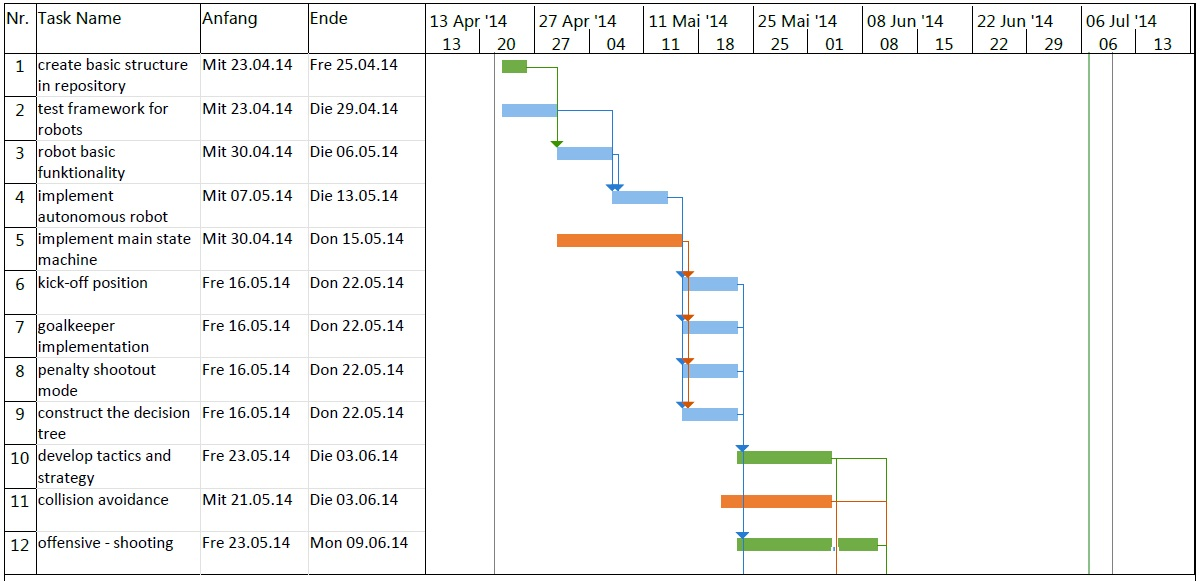
\includegraphics[width=\textwidth]{Pictures/ganttfinal1.jpg}
	\end{figure}
\end{frame}

\begin{frame}
	\frametitle{Gantt Chart II}
	\begin{figure}
		\centering
		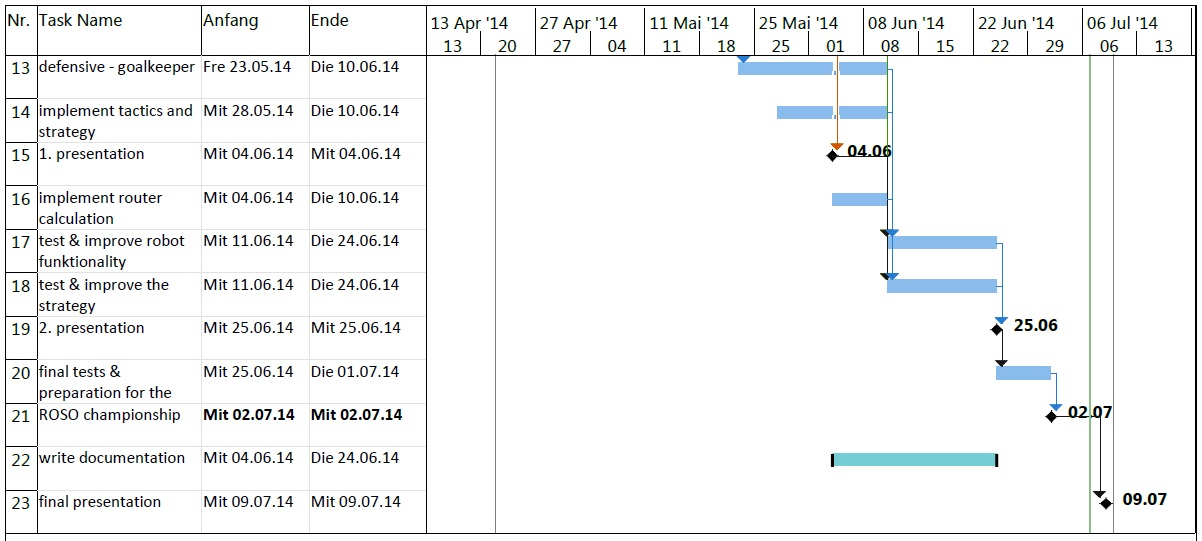
\includegraphics[width=\textwidth]{Pictures/ganttfinal2.jpg}
	\end{figure}
\end{frame}

\subsection{}
\begin{frame}
    \frametitle{Open Source}
    \textbf{Soon public available:}\\
    \textit{https://bitbucket.org/robosoccer/robosoccer}
    \begin{center}
        \begin{figure}
            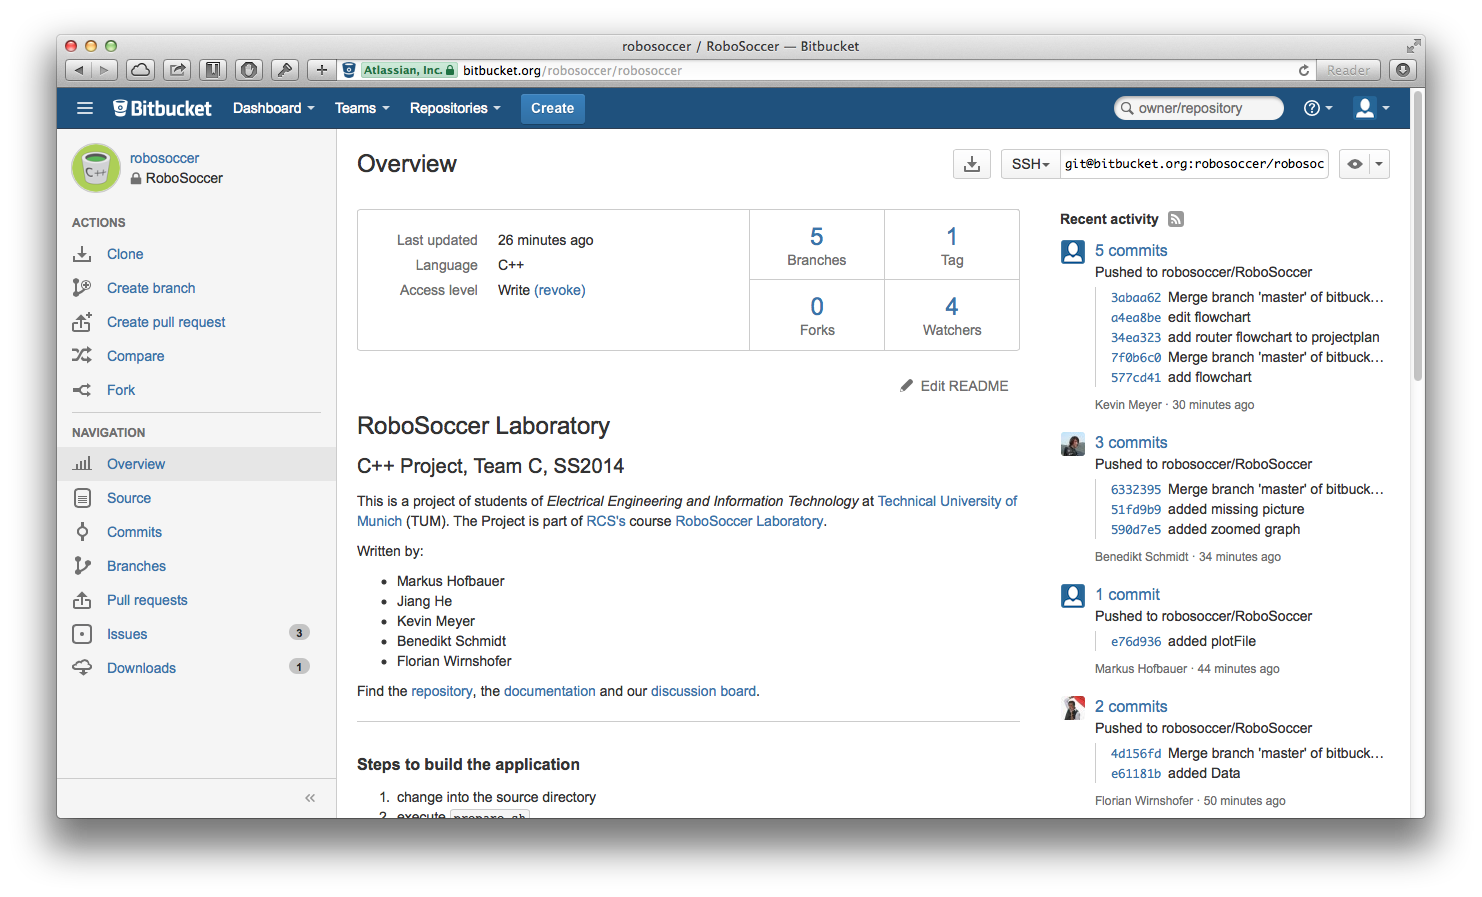
\includegraphics[width=0.8\textwidth]{bucket.png}
        \end{figure}
    \end{center}
\end{frame}

\subsection{Championship}
\begin{frame}
	\frametitle{We won the cup!}
	\begin{center}
	    \begin{figure}
	        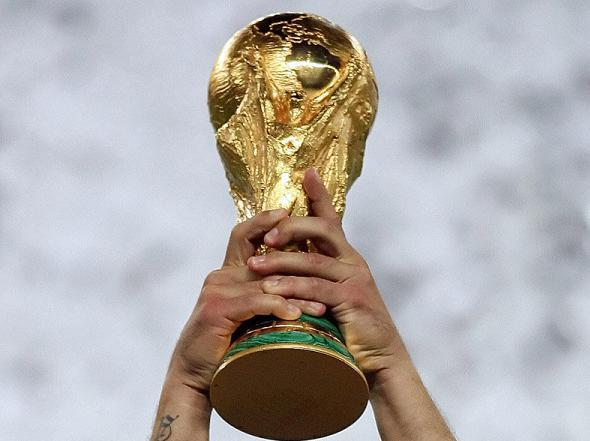
\includegraphics[width=0.8\textwidth]{wm}
	    \end{figure}
	\end{center}
\end{frame}

\subsection{Conclusion}
\begin{frame}
	\frametitle{Conclusion}
	\textbf{Resume and Proposals:}\\
	\begin{itemize}
		\item \textbf{Collision Avoidance:} potential controller instead of router
		\item \textbf{Strategy:} FSM instead of decision tree
		\item \textbf{Penalty:} goalkeeper position dependent of position of ball and kicker, before ball is kicked
		\item \textbf{Ball Control:} controller for dribbling skills
	\end{itemize}
\end{frame}

\section{}
\begin{frame}
	\hfill
	\begin{beamercolorbox}[shadow=true, rounded=true, wd=10cm]{presinative}
		\centering
		\Large{\textbf{Thank you for your attention!}}
	\end{beamercolorbox}
	\hfill \\
	\hfill \\
	\begin{block}{Some useless Facts}
		\begin{itemize}
			\item 29537 lines of code					% 28207 + 1530 	gui
			\item 107 classes ($+$ 19 mock classes and 74 test classes)	% 100 	+ 7 	gui
			\item 1452 commits						% 1394	+ 59	gui
			\item 778 unit tests
			\item 118 issues (on \textit{bitbucket.org})
			\item 1.23 MB per minute logging output
			\item This presentation has 57 slides (1457 lines of \LaTeX\ Beamer)
		\end{itemize}
	\end{block}
\end{frame}

\end{document}
